\section*{\sffamily \Large Results with constant permitivitty}

\subsection*{\sffamily \large Convergence of a spherical cavity}
\begin{itemize}
    \item Show convergence to analytical solution for
    \begin{itemize}
        \item BEM-BEM
\begin{figure}[!htb]
\minipage{0.32\textwidth}
  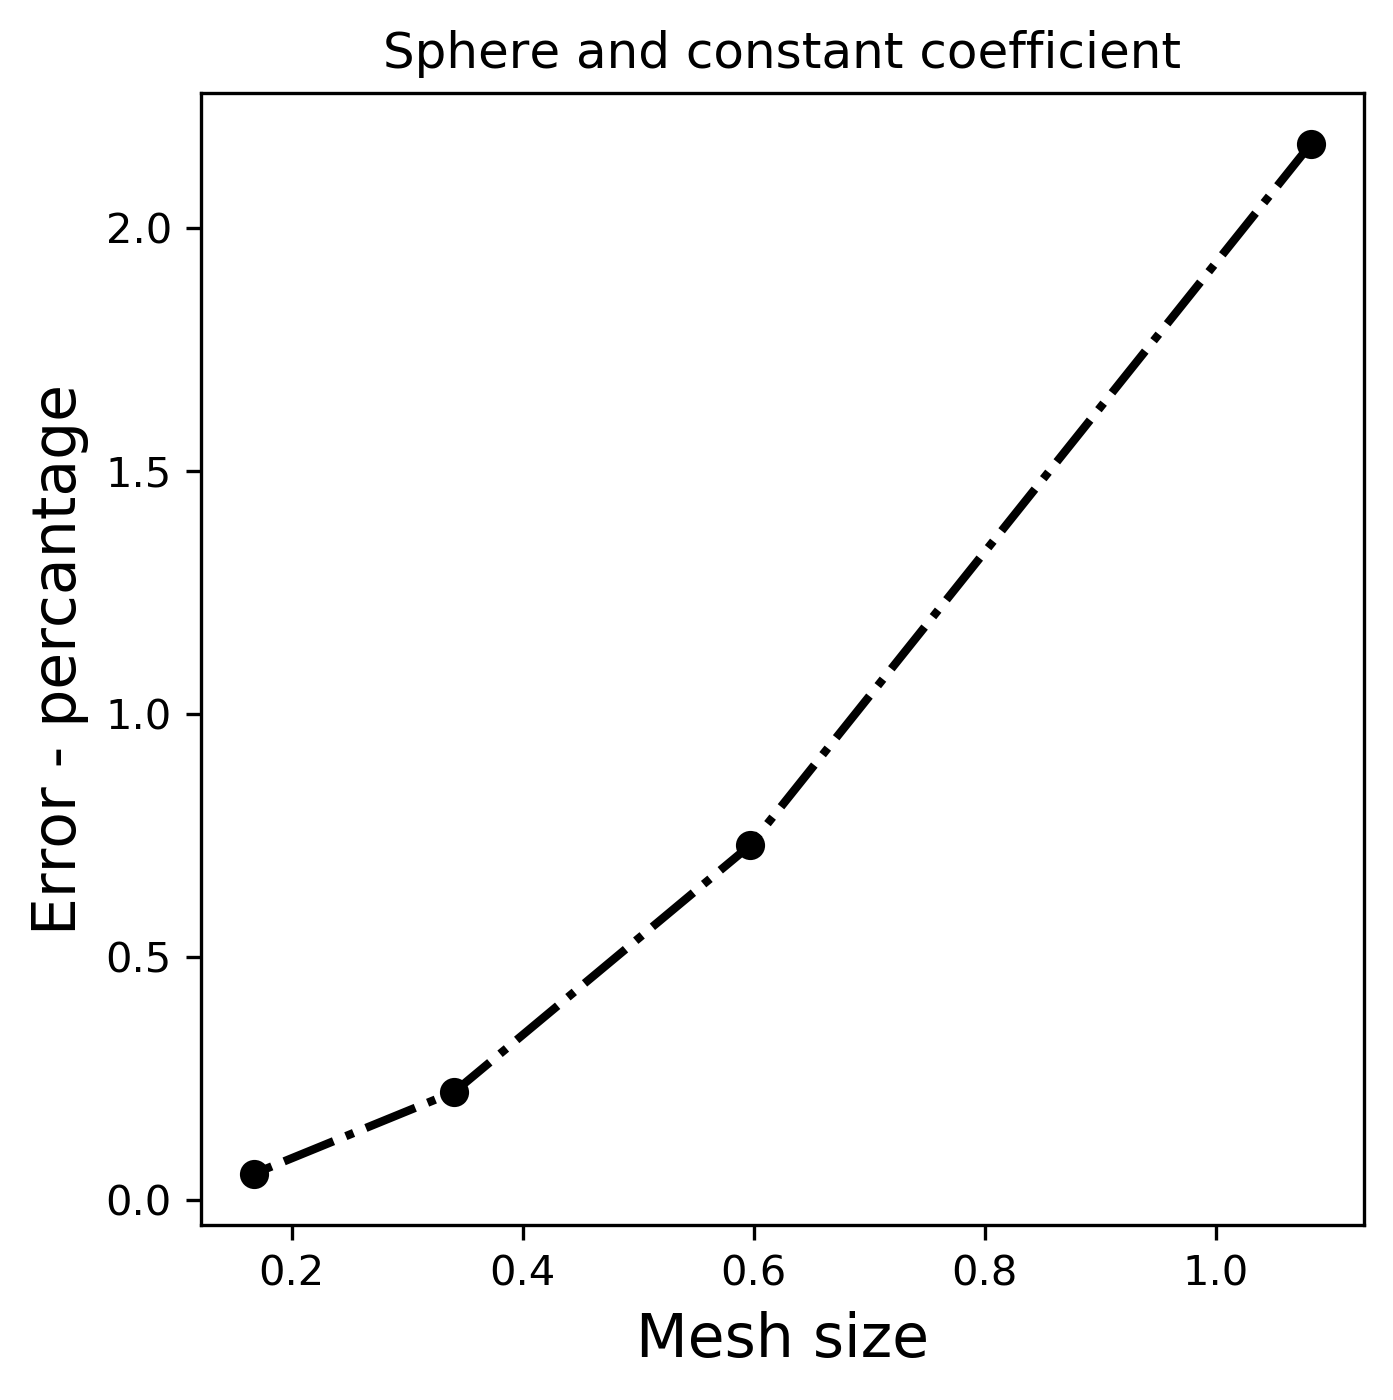
\includegraphics[width=\linewidth]{BEM_BEM_Sphere_const_coeff_error.png}
  \caption{Error}
\endminipage\hfill
\minipage{0.32\textwidth}
  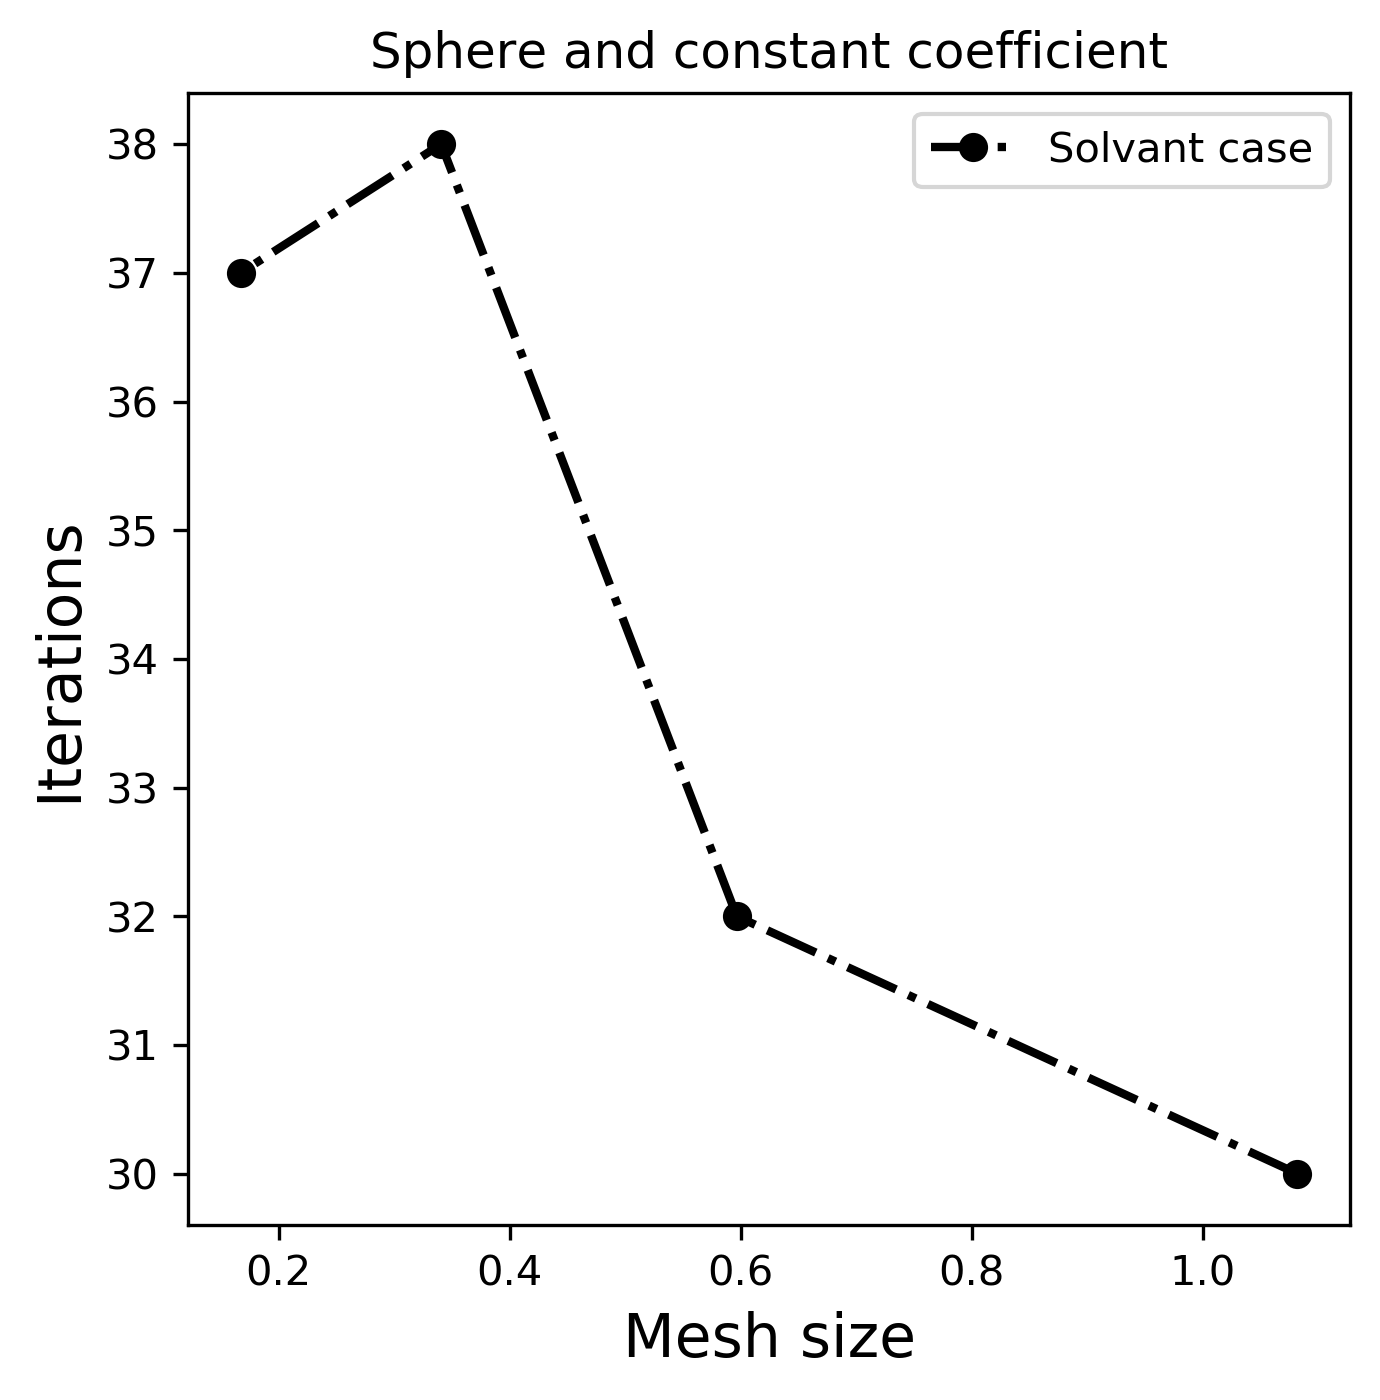
\includegraphics[width=\linewidth]{BEM_BEM_Sphere_const_coeff_iter.png}
  \caption{Iterations}
\endminipage\hfill
\minipage{0.32\textwidth}%
  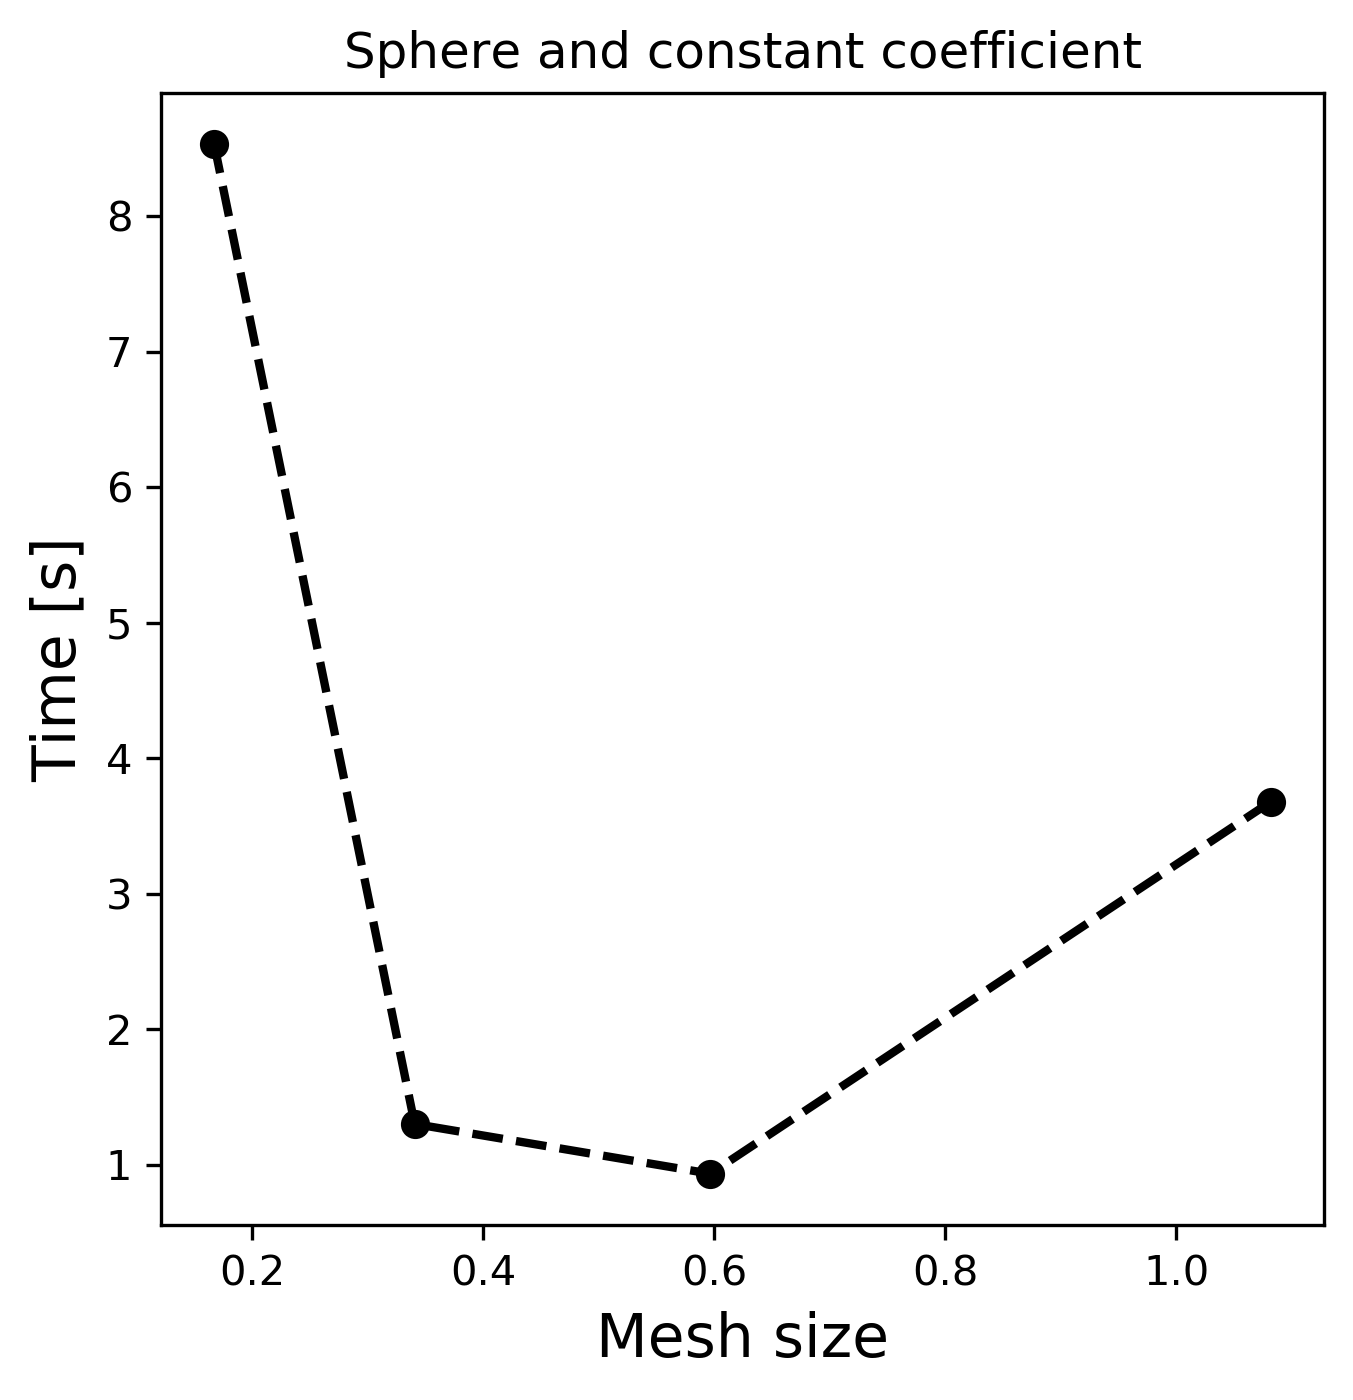
\includegraphics[width=\linewidth]{BEM_BEM_Sphere_const_coeff_time.png}
  \caption{Computational time}
\endminipage
\end{figure}
        \item Standard FEM-BEM
\begin{figure}[!htb]
\minipage{0.32\textwidth}
  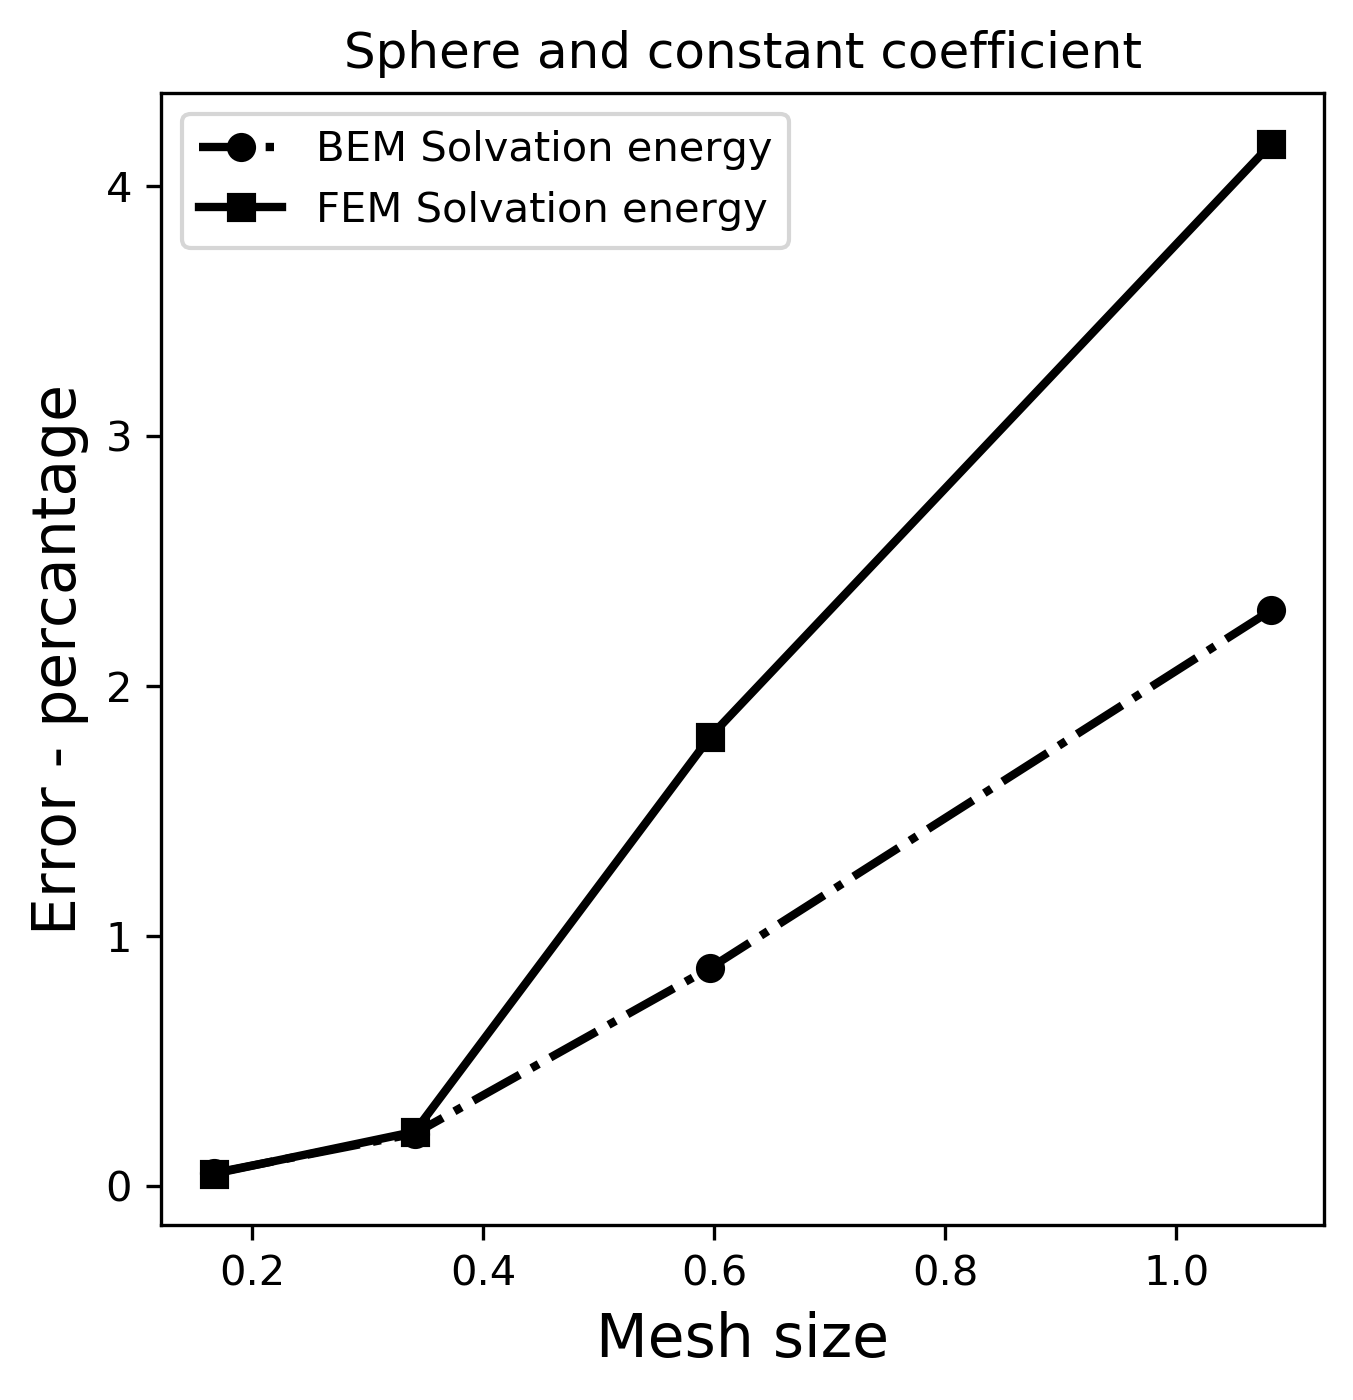
\includegraphics[width=\linewidth]{FEM_BEM_Sphere_const_coeff_error.png}
  \caption{Error}
\endminipage\hfill
\minipage{0.32\textwidth}
  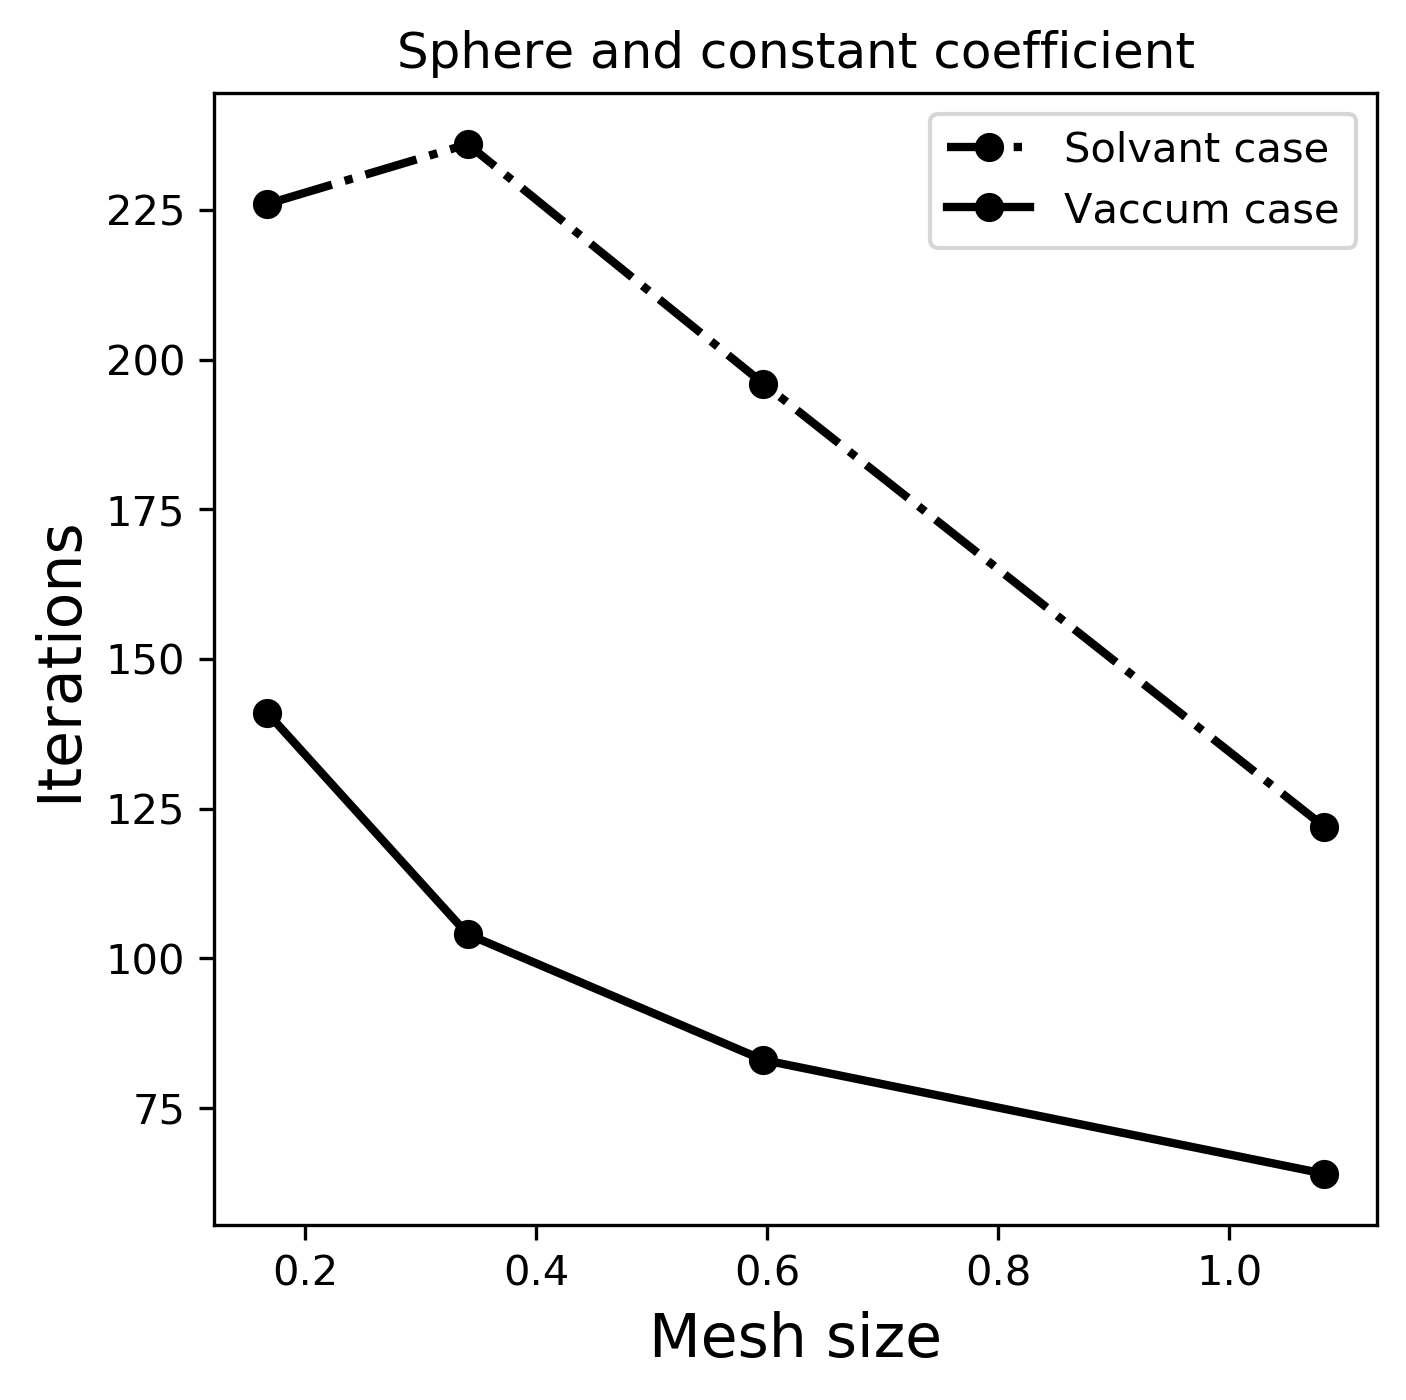
\includegraphics[width=\linewidth]{FEM_BEM_Sphere_const_coeff_iter.png}
  \caption{Iterations}
\endminipage\hfill
\minipage{0.32\textwidth}%
  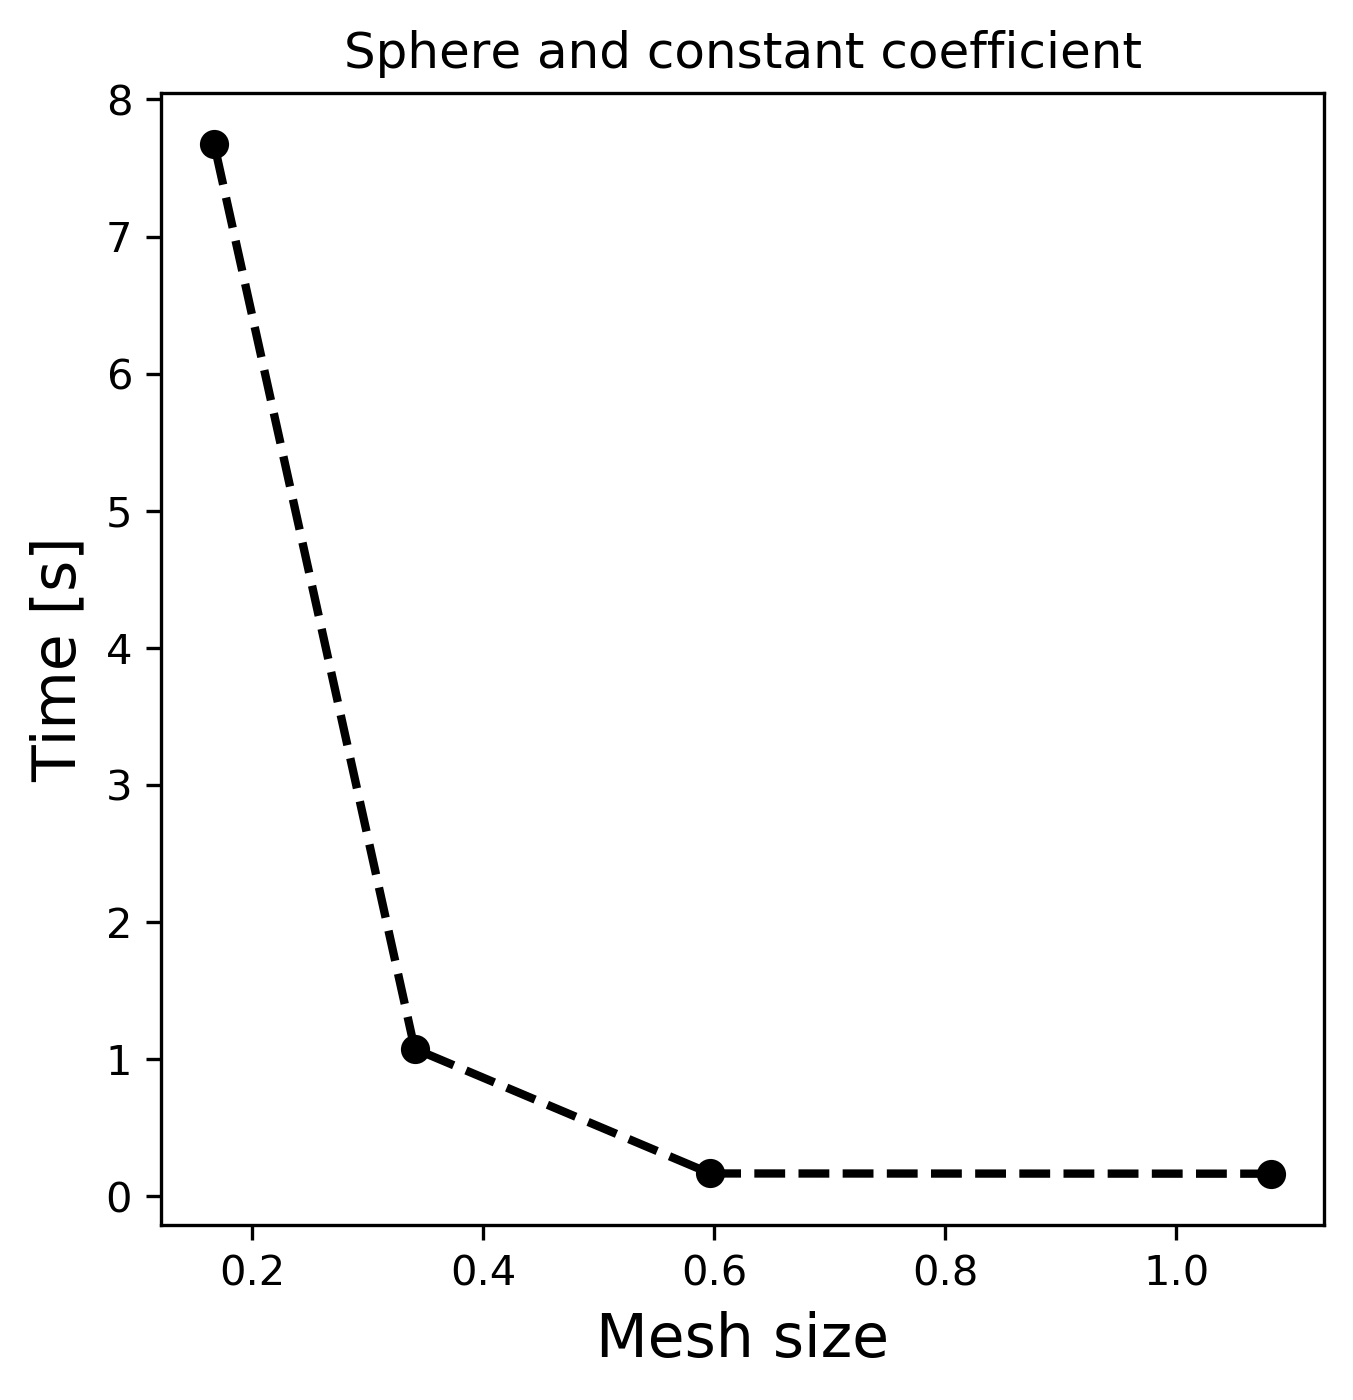
\includegraphics[width=\linewidth]{FEM_BEM_Sphere_const_coeff_time.png}
  \caption{Computational time}
\endminipage
\end{figure}
        \item Hybrid FEM-BEM
\begin{figure}[!htb]
\minipage{0.32\textwidth}
  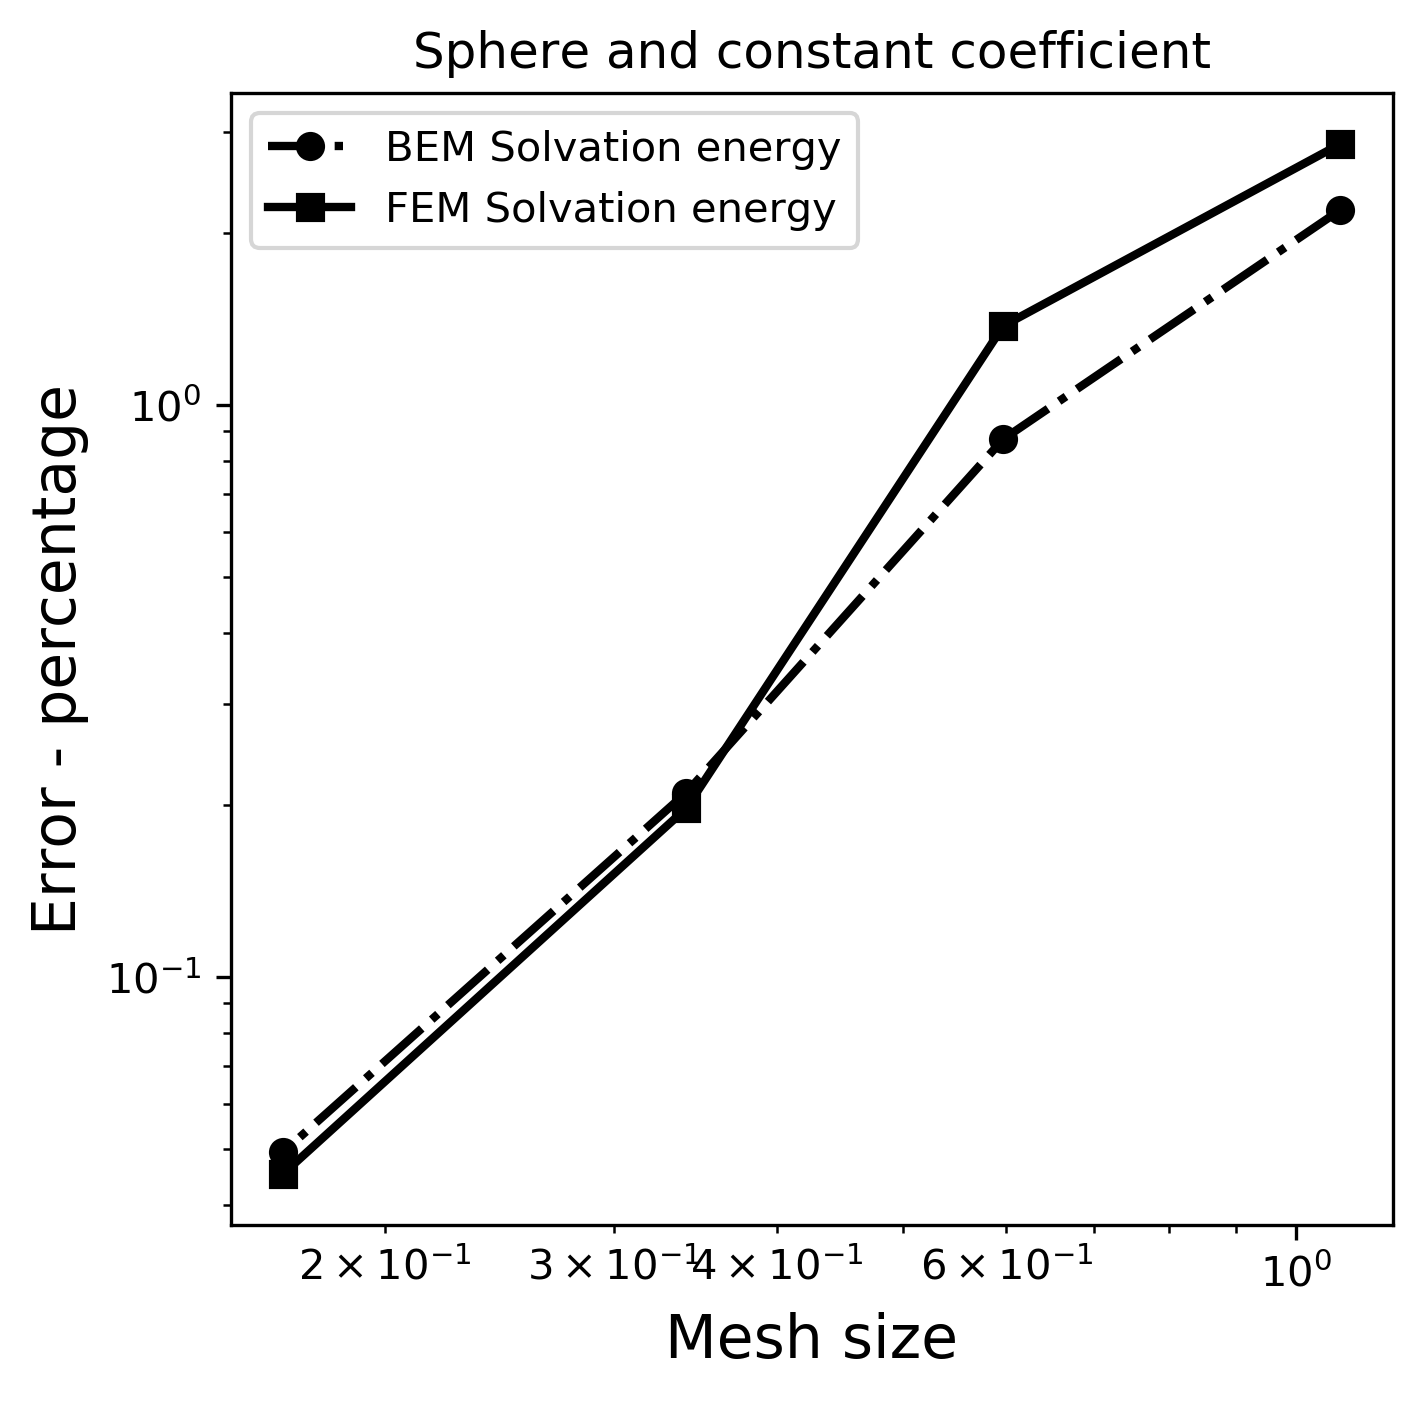
\includegraphics[width=\linewidth]{Hybrid_FEM_BEM_Sphere_const_coeff_error.png}
  \caption{Error}
\endminipage\hfill
\minipage{0.32\textwidth}
  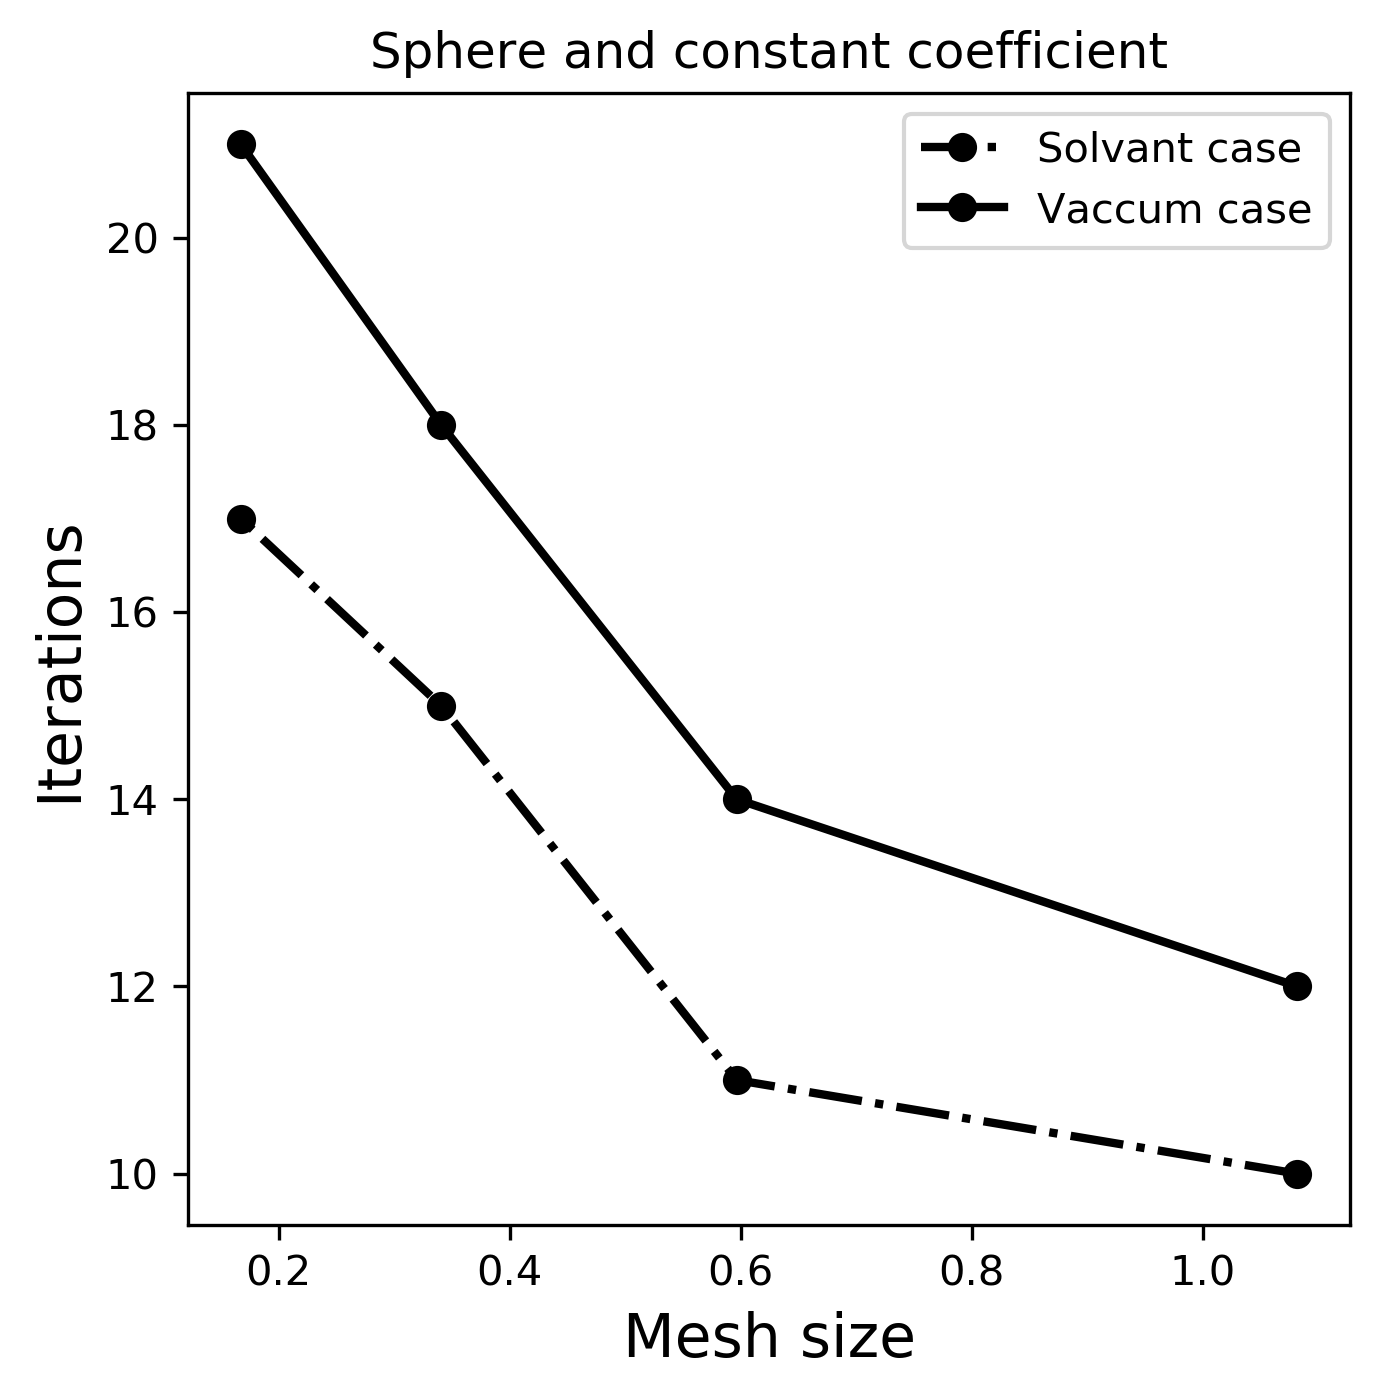
\includegraphics[width=\linewidth]{Hybrid_FEM_BEM_Sphere_const_coeff_iter.png}
  \caption{Iterations}
\endminipage\hfill
\minipage{0.32\textwidth}%
  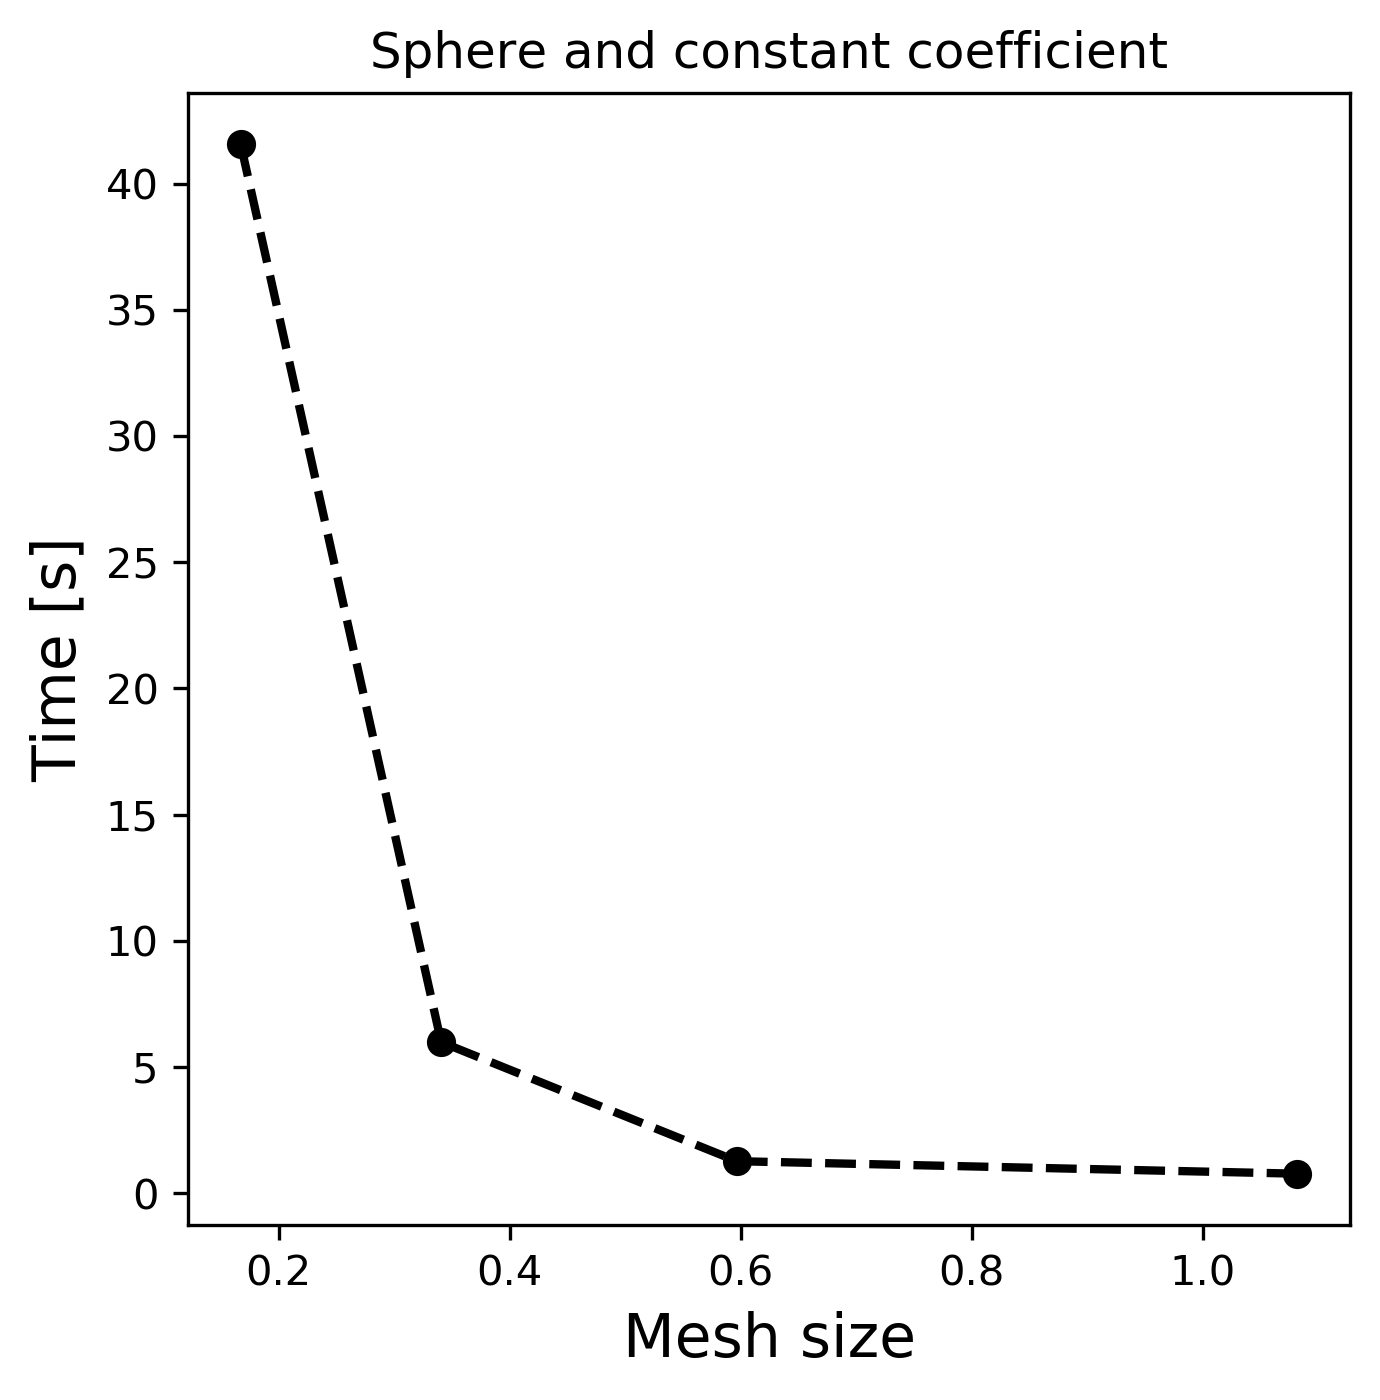
\includegraphics[width=\linewidth]{Hybrid_FEM_BEM_Sphere_const_coeff_time.png}
  \caption{Computational time}
\endminipage
\end{figure}
    \end{itemize}
\end{itemize}

\subsection*{\sffamily \large Performance for a molecular geometry}
\begin{itemize}
    \item Use arginine or a small protein (1PGB?)
    \begin{itemize}
        \item BEM-BEM
\begin{figure}[!htb]
\minipage{0.45\textwidth}
  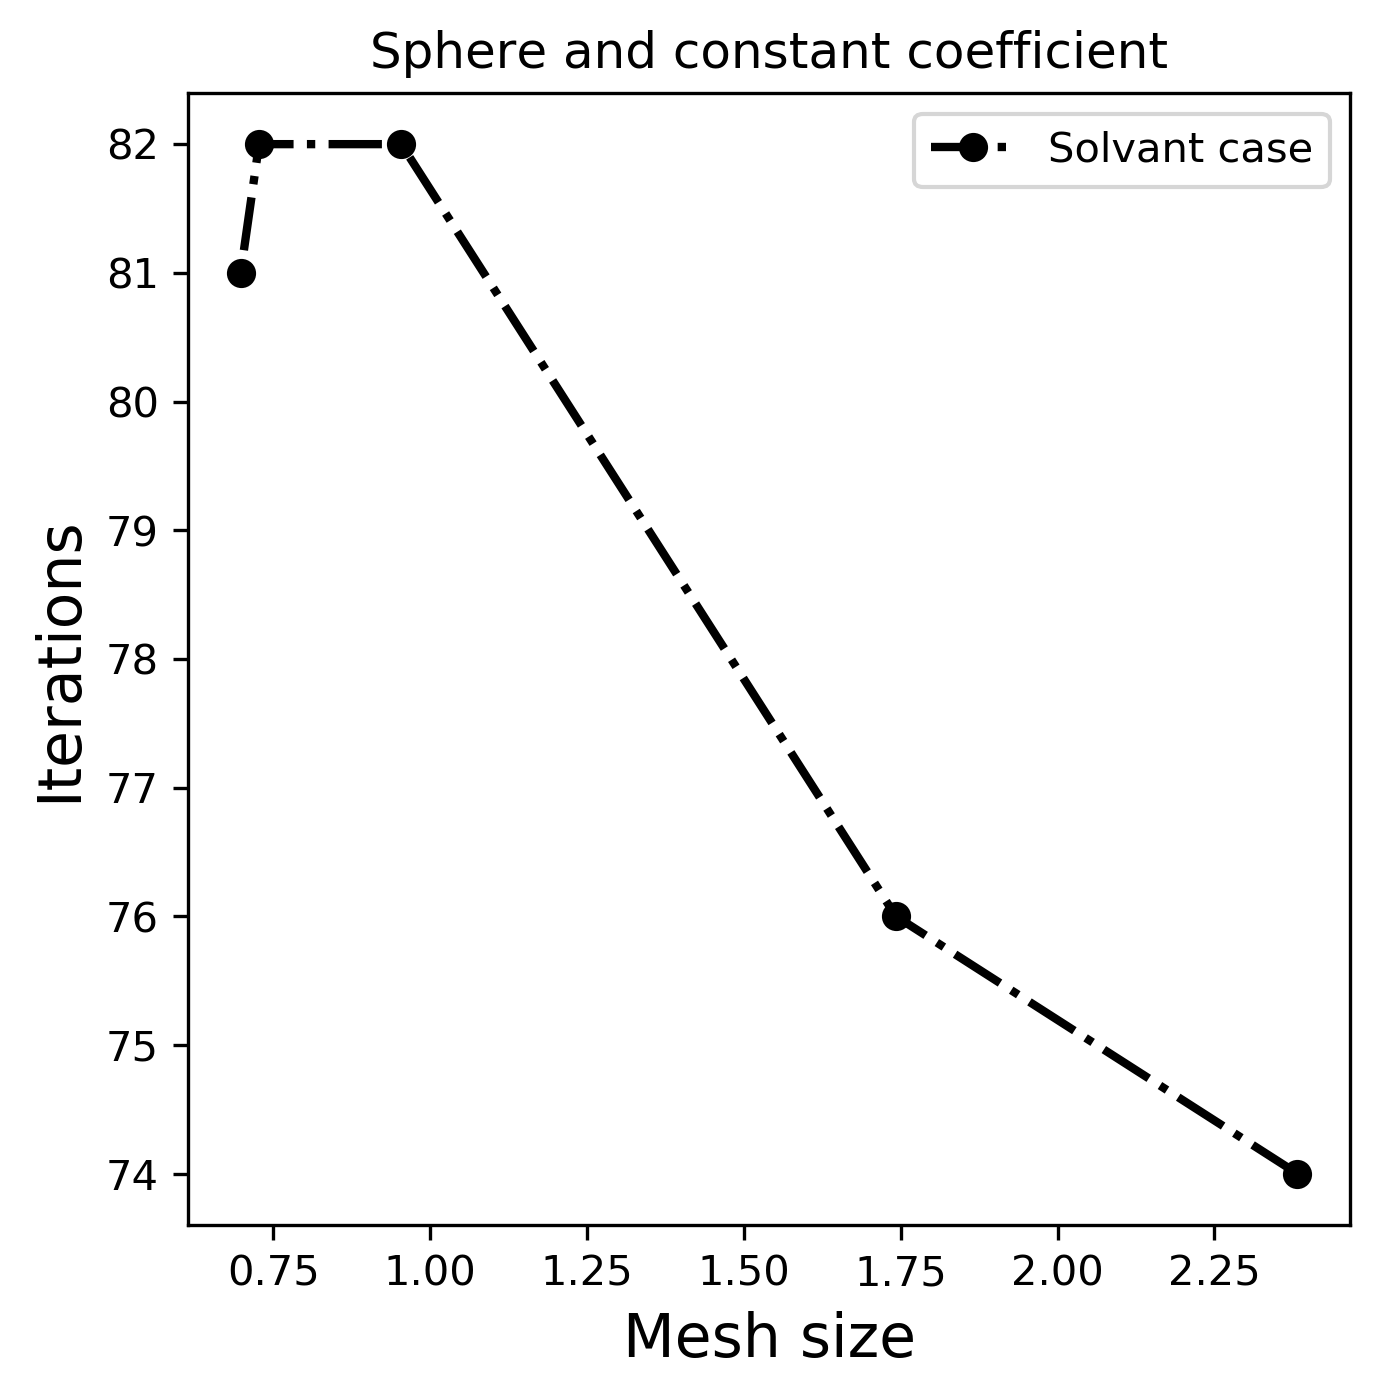
\includegraphics[width=\linewidth]{BEM_BEM_Arginine_const_coeff_iter.png}
  \caption{Iterations}
\endminipage\hfill
\minipage{0.45\textwidth}%
  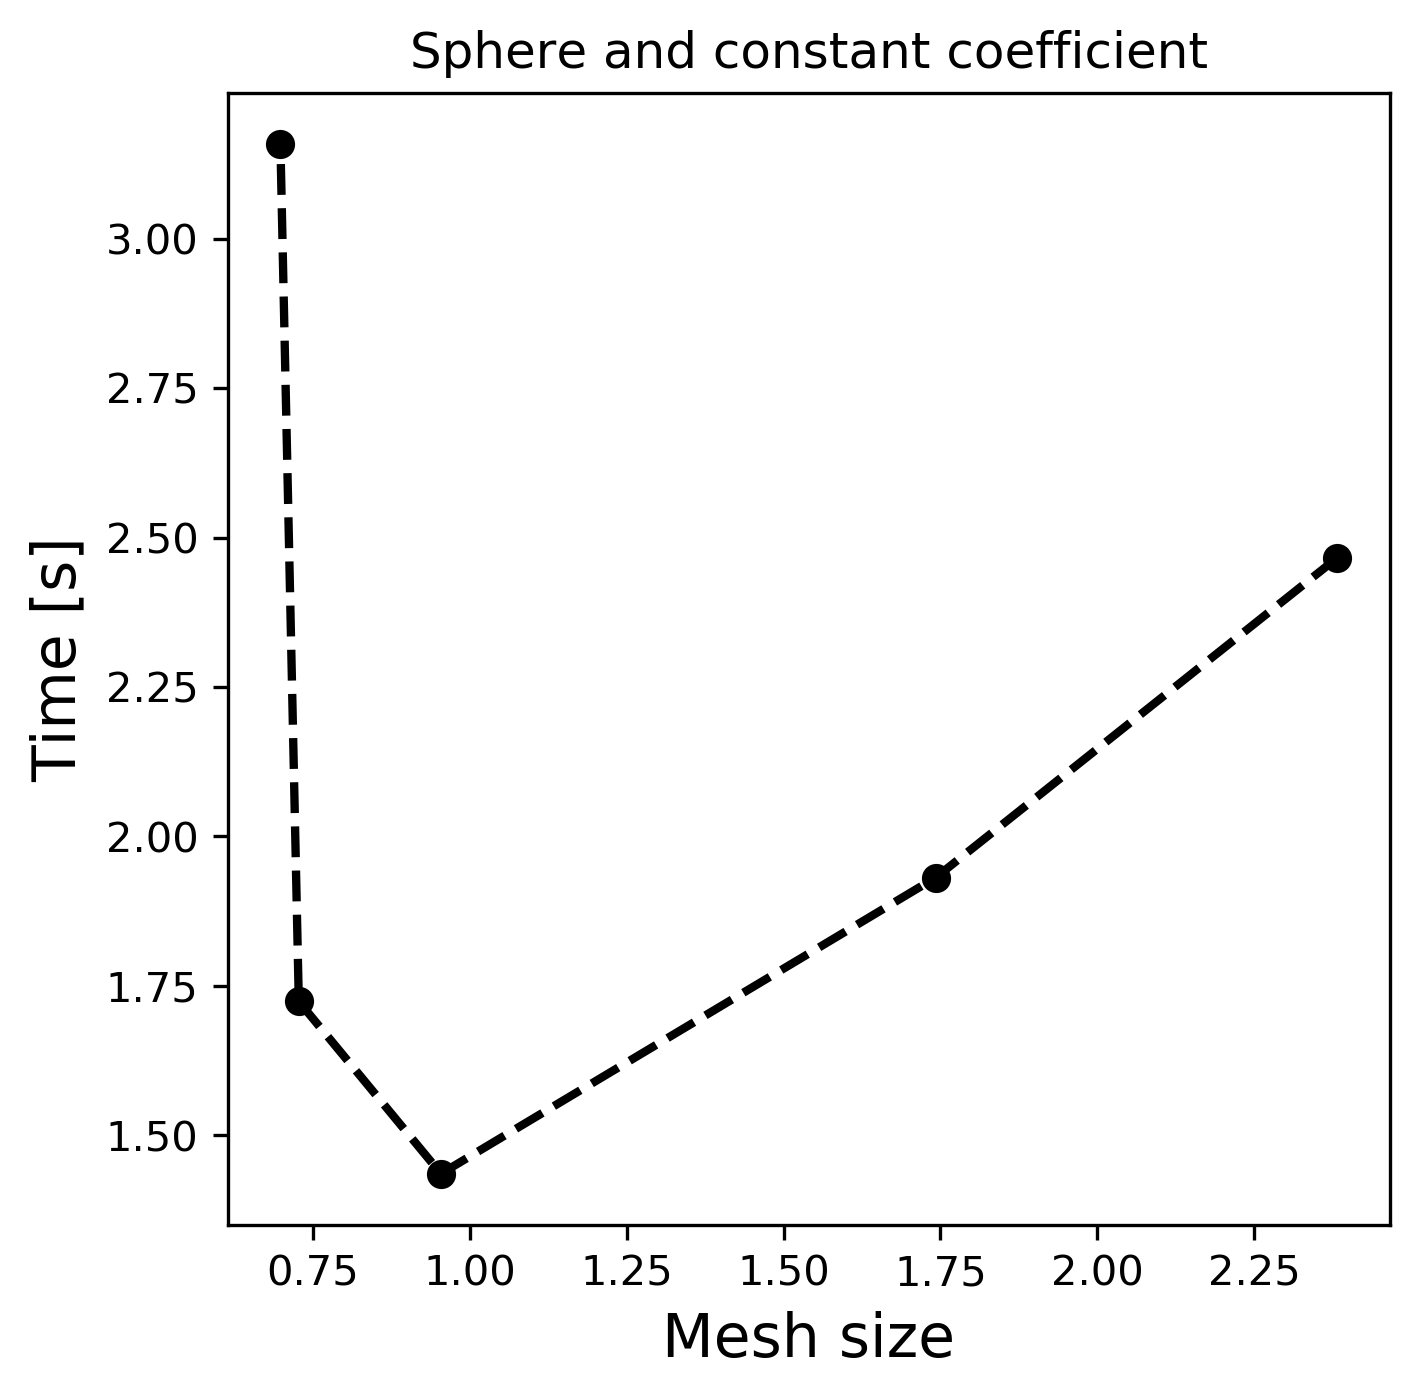
\includegraphics[width=\linewidth]{BEM_BEM_Arginine_const_coeff_time.png}
  \caption{Computational time}
\endminipage
\end{figure}
        \item Standard FEM-BEM
\begin{figure}[!htb]
\minipage{0.45\textwidth}
  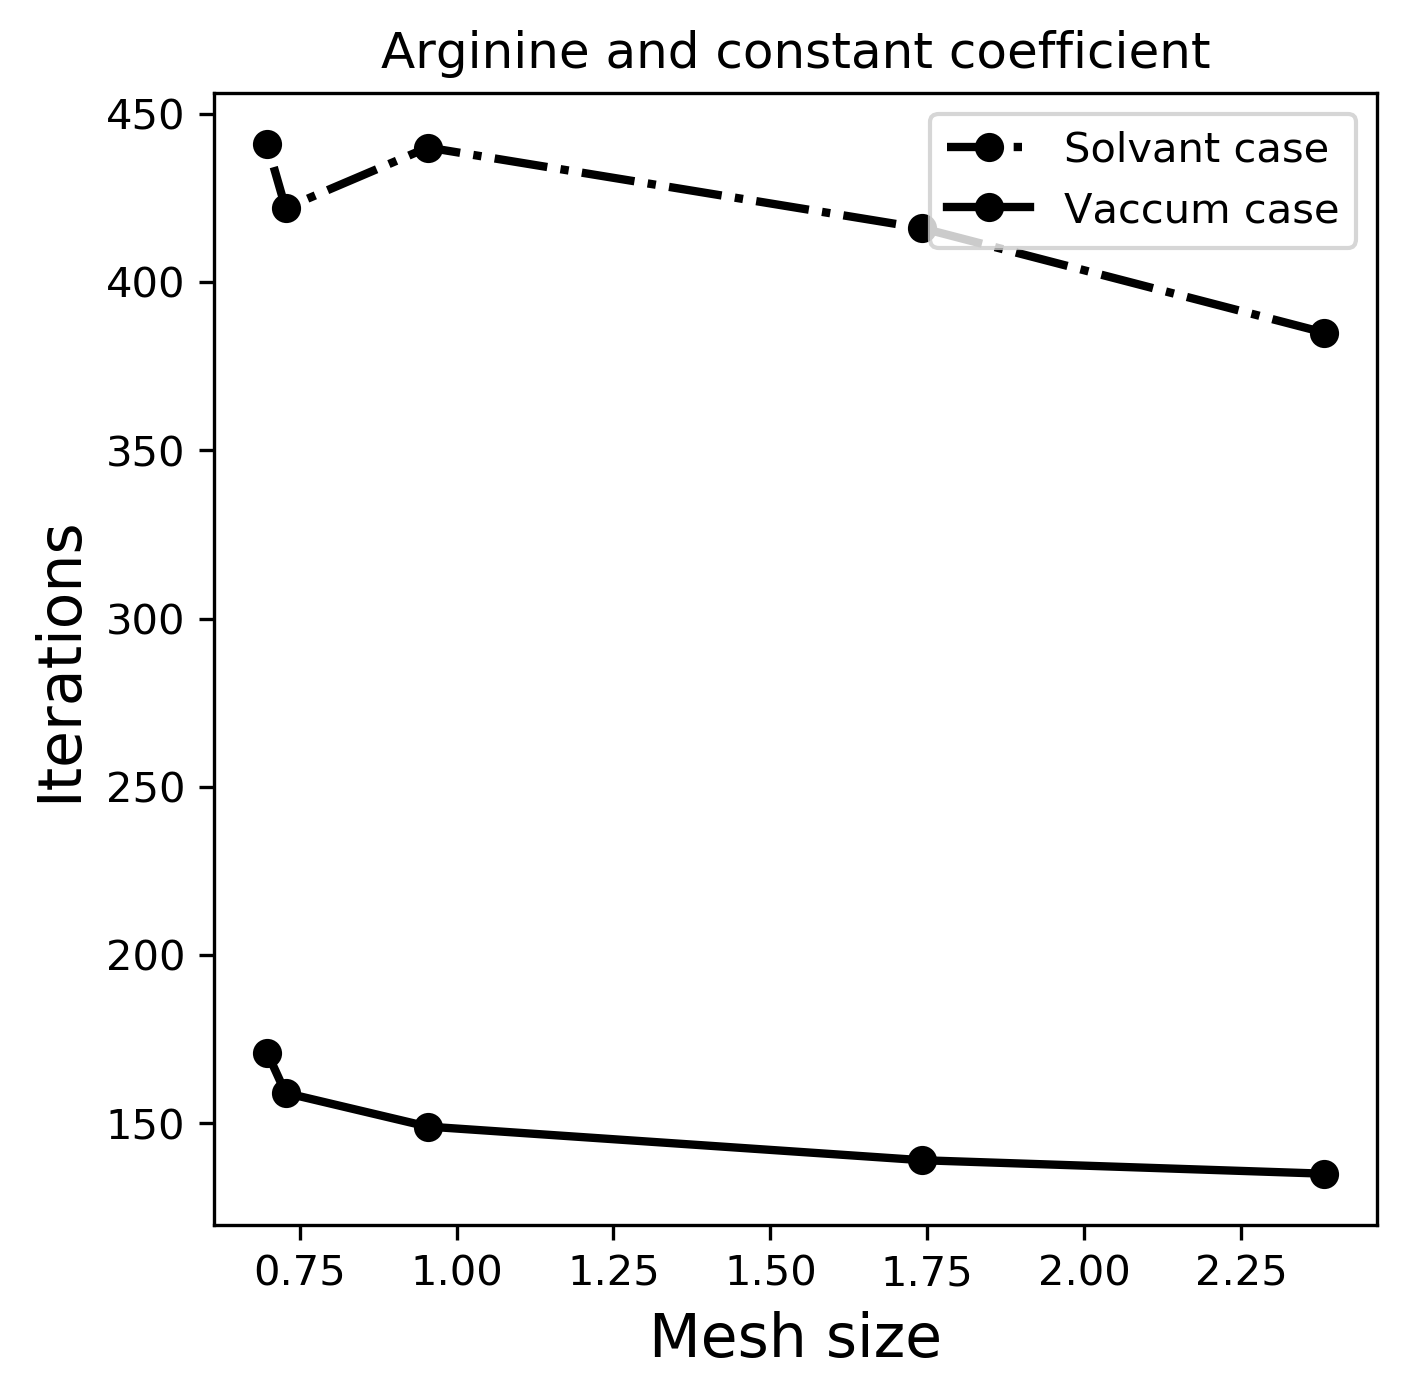
\includegraphics[width=\linewidth]{FEM_BEM_Arginine_const_coeff_iter.png}
  \caption{Iterations}
\endminipage\hfill
\minipage{0.45\textwidth}%
  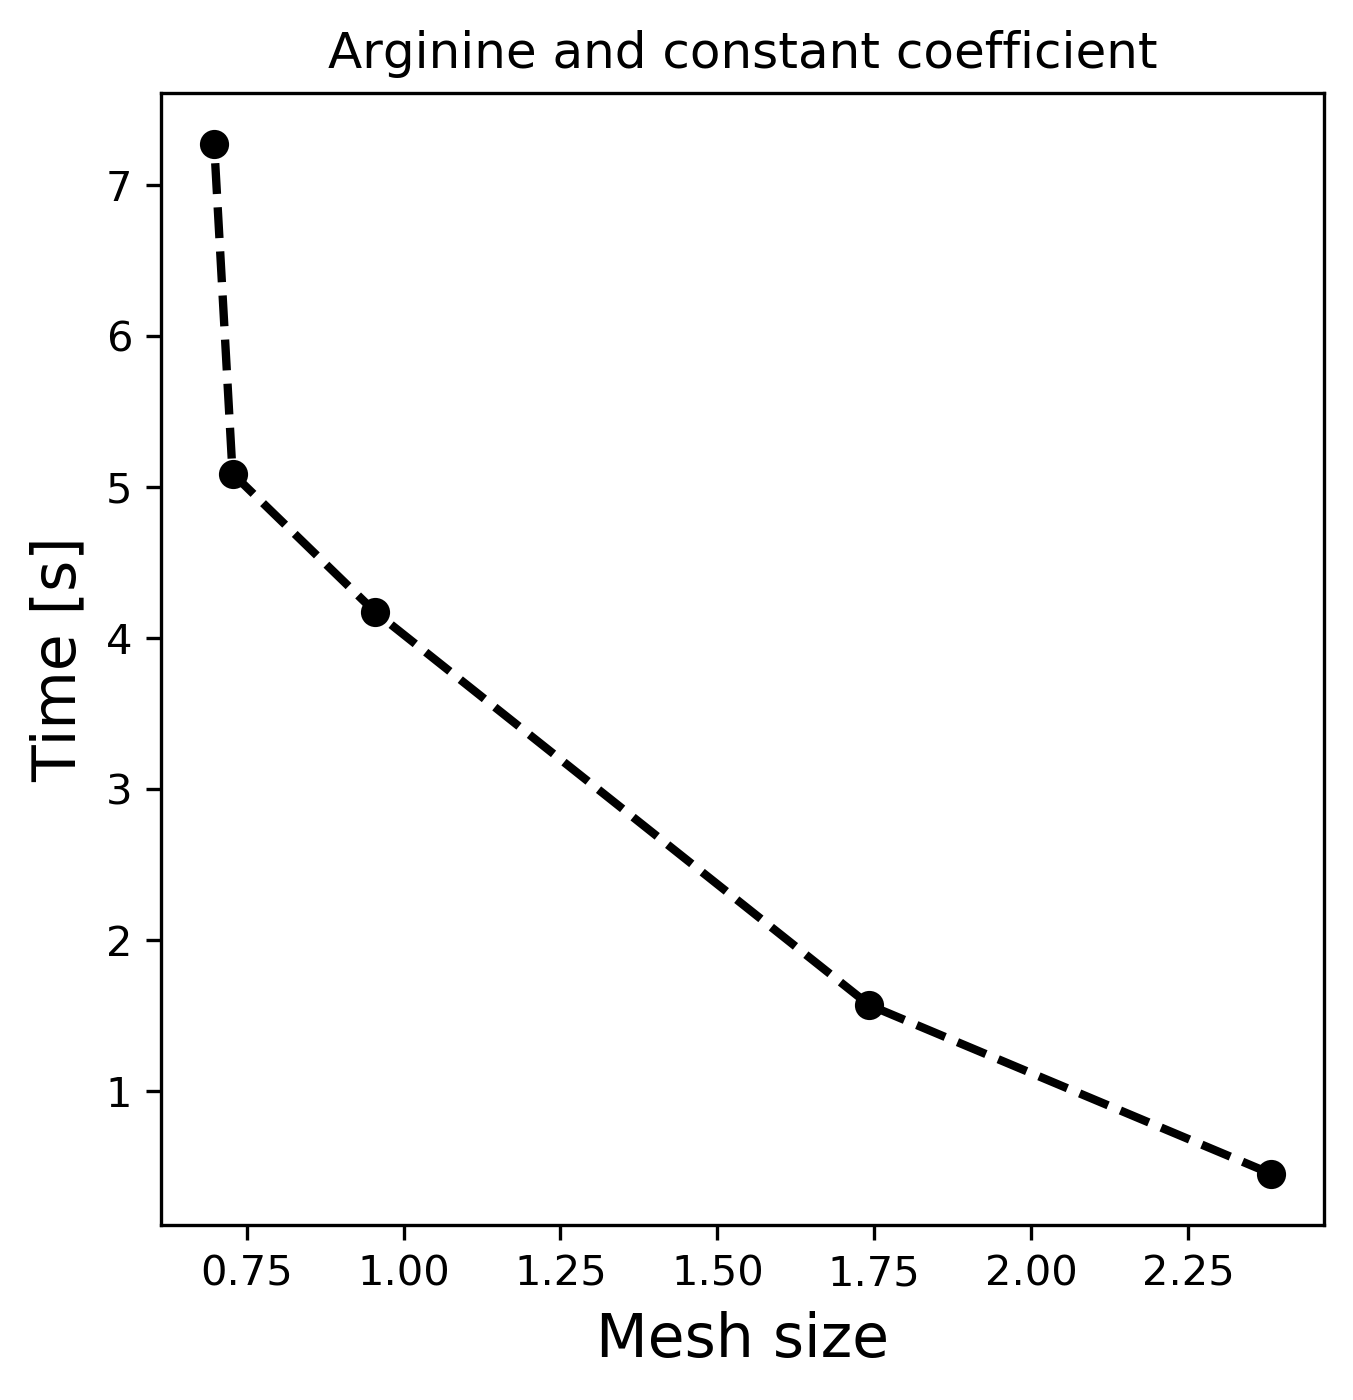
\includegraphics[width=\linewidth]{FEM_BEM_Arginine_const_coeff_time.png}
  \caption{Computational time}
\endminipage
\end{figure}
        \item Hybrid FEM-BEM
\begin{figure}[!htb]
\minipage{0.45\textwidth}
  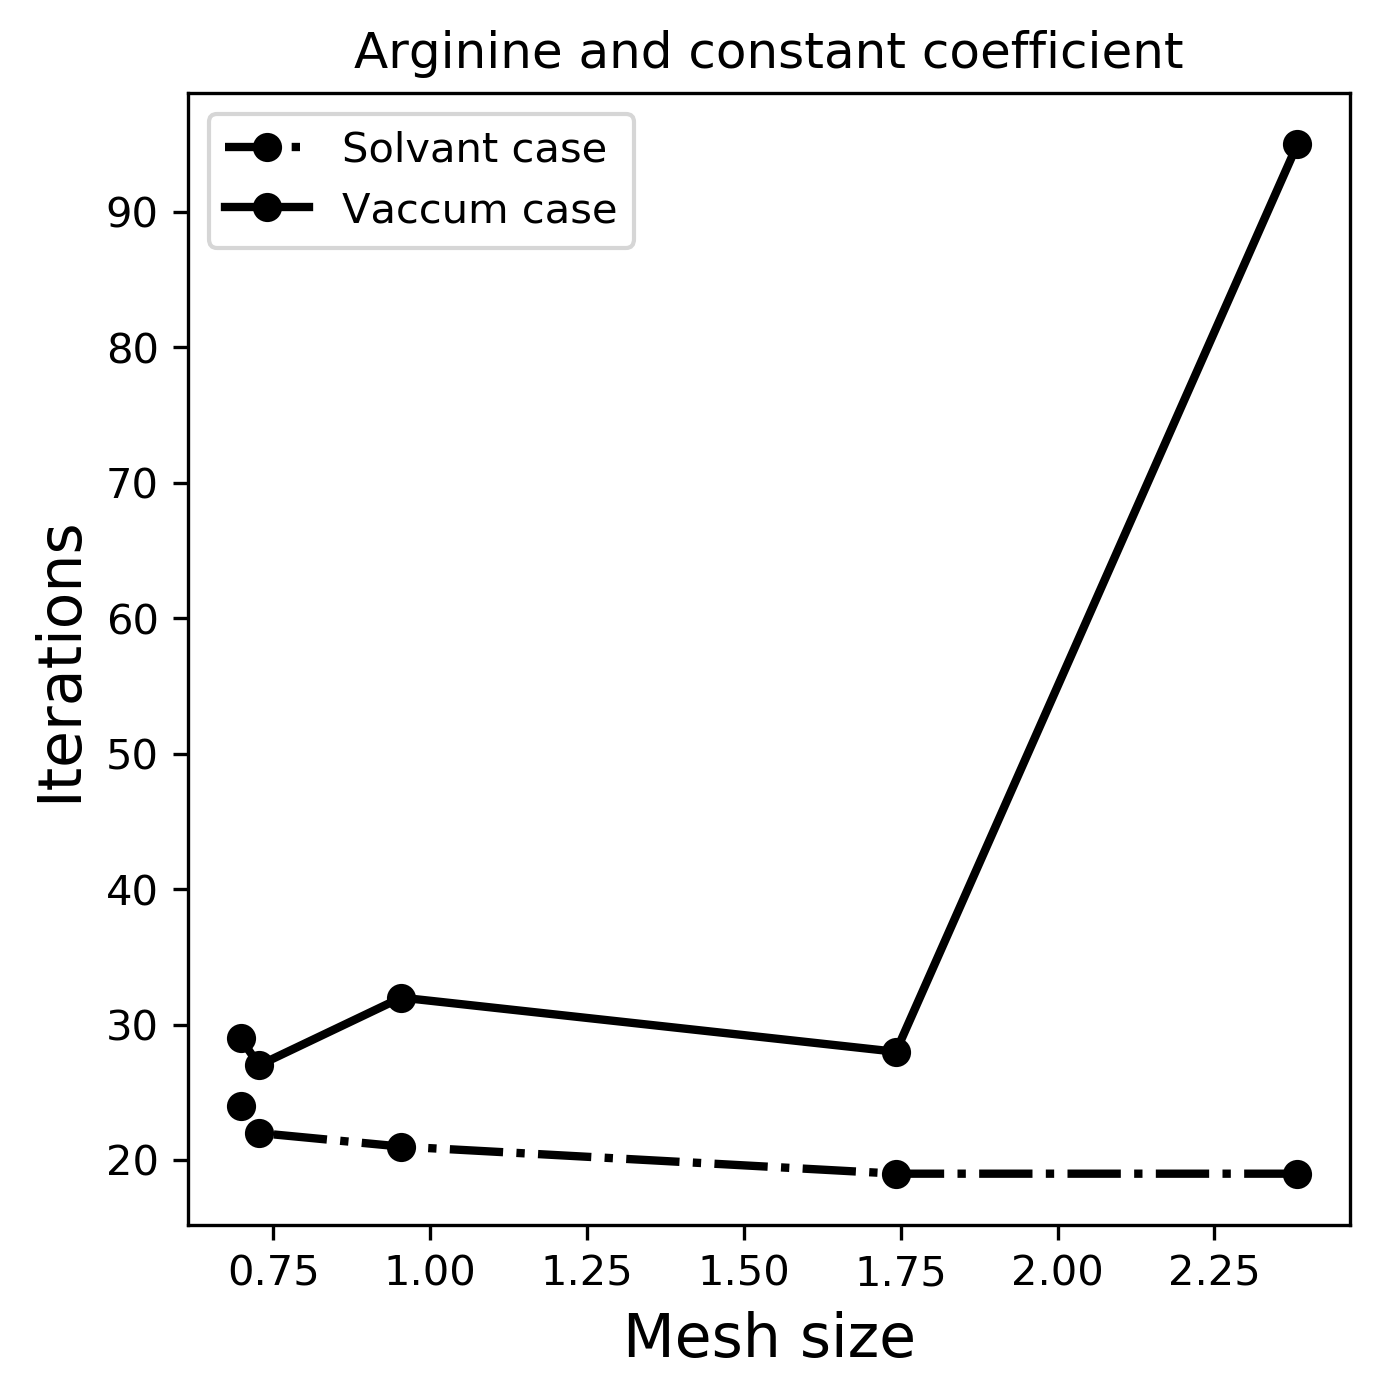
\includegraphics[width=\linewidth]{Hybrid_FEM_BEM_Arginine_const_coeff_iter.png}
  \caption{Iterations}
\endminipage\hfill
\minipage{0.45\textwidth}%
  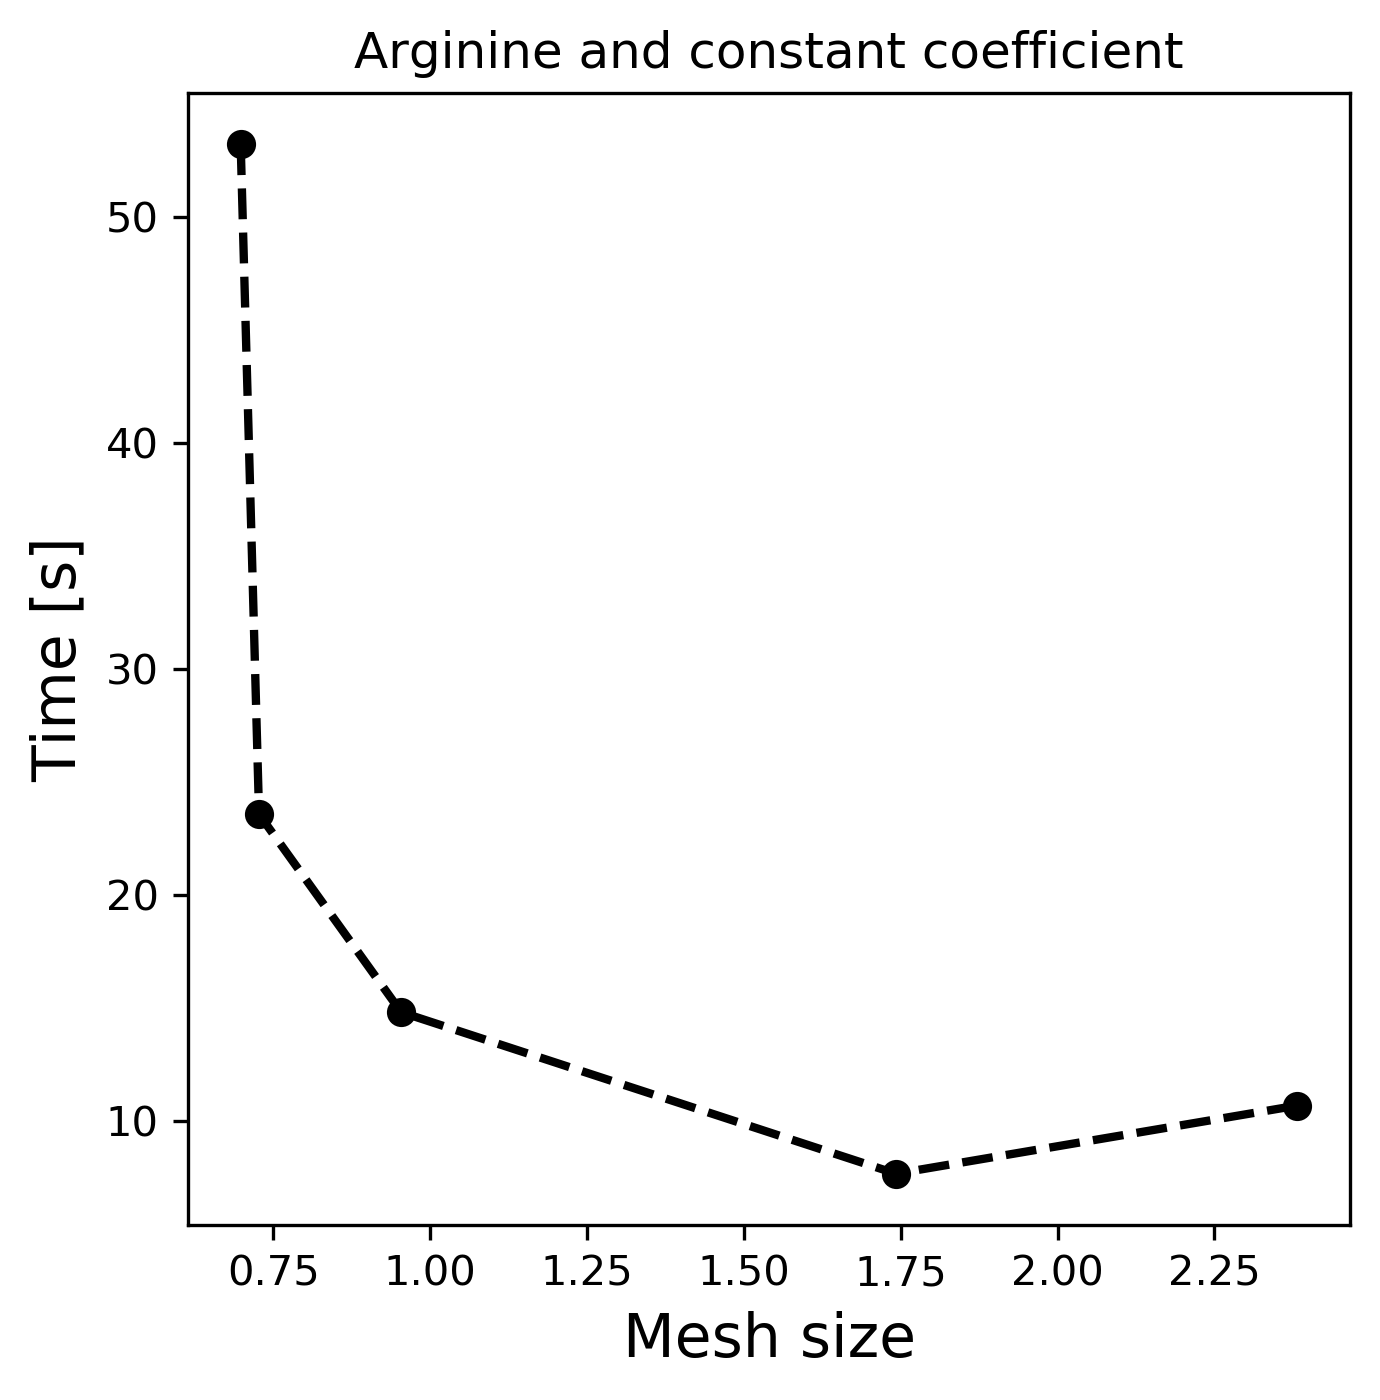
\includegraphics[width=\linewidth]{Hybrid_FEM_BEM_Arginine_const_coeff_time.png}
  \caption{Computational time}
\endminipage
\end{figure}
    \end{itemize}
    \item Compare computer time and iterations for FEM-BEM with standard and hybrid approaches, without preconditioner. Choose hybrid.
    \item Show performance of hybrid method with preconditioner.
\end{itemize}

\section*{\sffamily \Large Results with variable permittivity}

\begin{table}
\centering
\begin{tabular}{c|c|c}
&Mesh size & $\Delta G_{solv}$\\
&\AA       &  kcal/mol \\
\hline
\multirow{3}{*}{APBS}& 0.39$\times$0.39$\times$0.39 & -32.4042\\ 
&0.26$\times$0.26$\times$0.26 & -32.3375\\ 
&0.17$\times$0.17$\times$0.17 & -32.3413\\ 
\hline
&Mesh dens. & \\
&vert/\AA$^2$ & \\
\hline
%\multirow{5}{*}{Standard FEM-BEM}& 2 & -36.239\\
    & 2 & -36.239\\
Standard    & 4  & -33.129 \\
FEM-BEM    & 8  & -32.674 \\
    & 12 & -32.648 \\
    & 16 & -32.293 \\
\hline
%\multirow{5}{*}{Standard FEM-BEM}& 2 & -29.554\\
    & 2 & -29.554\\
Hybrid    & 4  & -33.766 \\
FEM-BEM    & 8  & -32.586 \\
    & 12 & -32.891 \\
    & 16 & -32.528 \\
\hline
\end{tabular}
\caption{}
\end{table}

    \begin{itemize}
        \item Standard FEM-BEM
\begin{figure}[!htb]
\minipage{0.45\textwidth}
  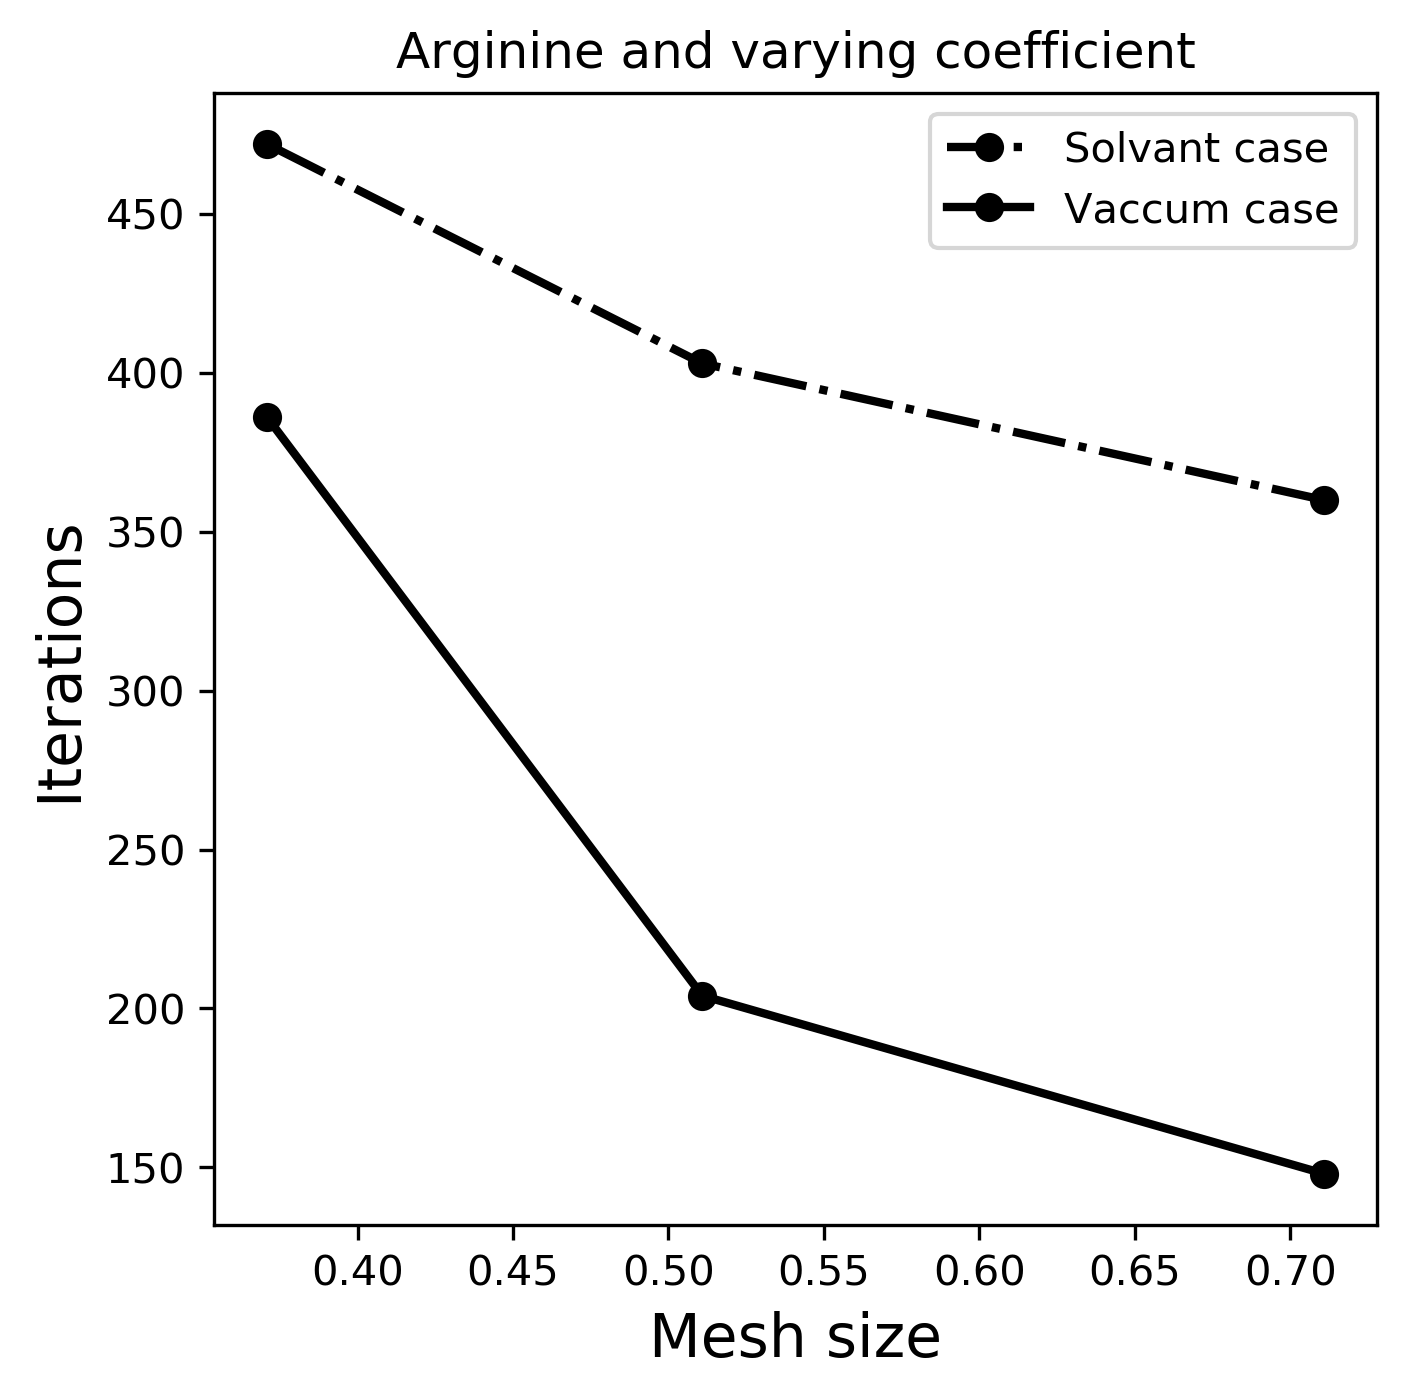
\includegraphics[width=\linewidth]{FEM_BEM_Sphere_varying_coeff_iter.png}
  \caption{Iterations}
\endminipage\hfill
\minipage{0.45\textwidth}%
  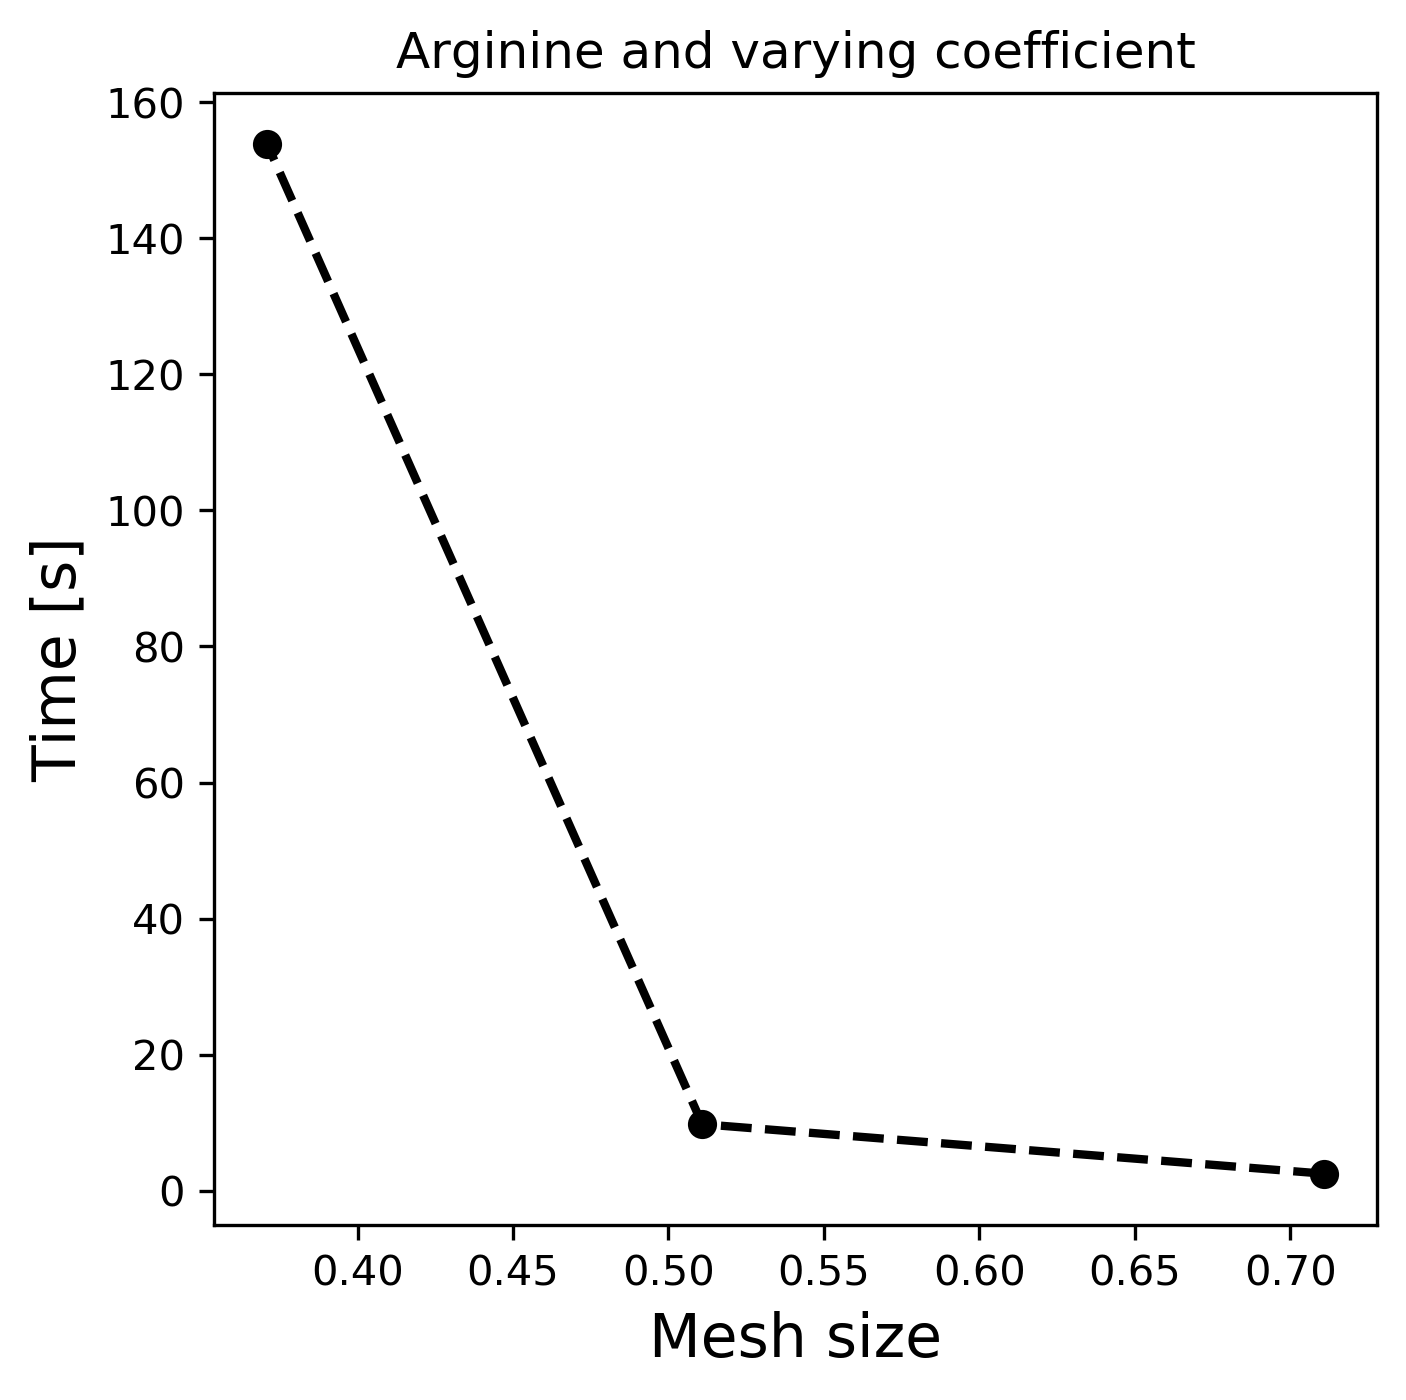
\includegraphics[width=\linewidth]{FEM_BEM_Sphere_varying_coeff_time.png}
  \caption{Computational time}
\endminipage
\end{figure}
        \item Hybrid FEM-BEM
\begin{figure}[!htb]
\minipage{0.45\textwidth}
  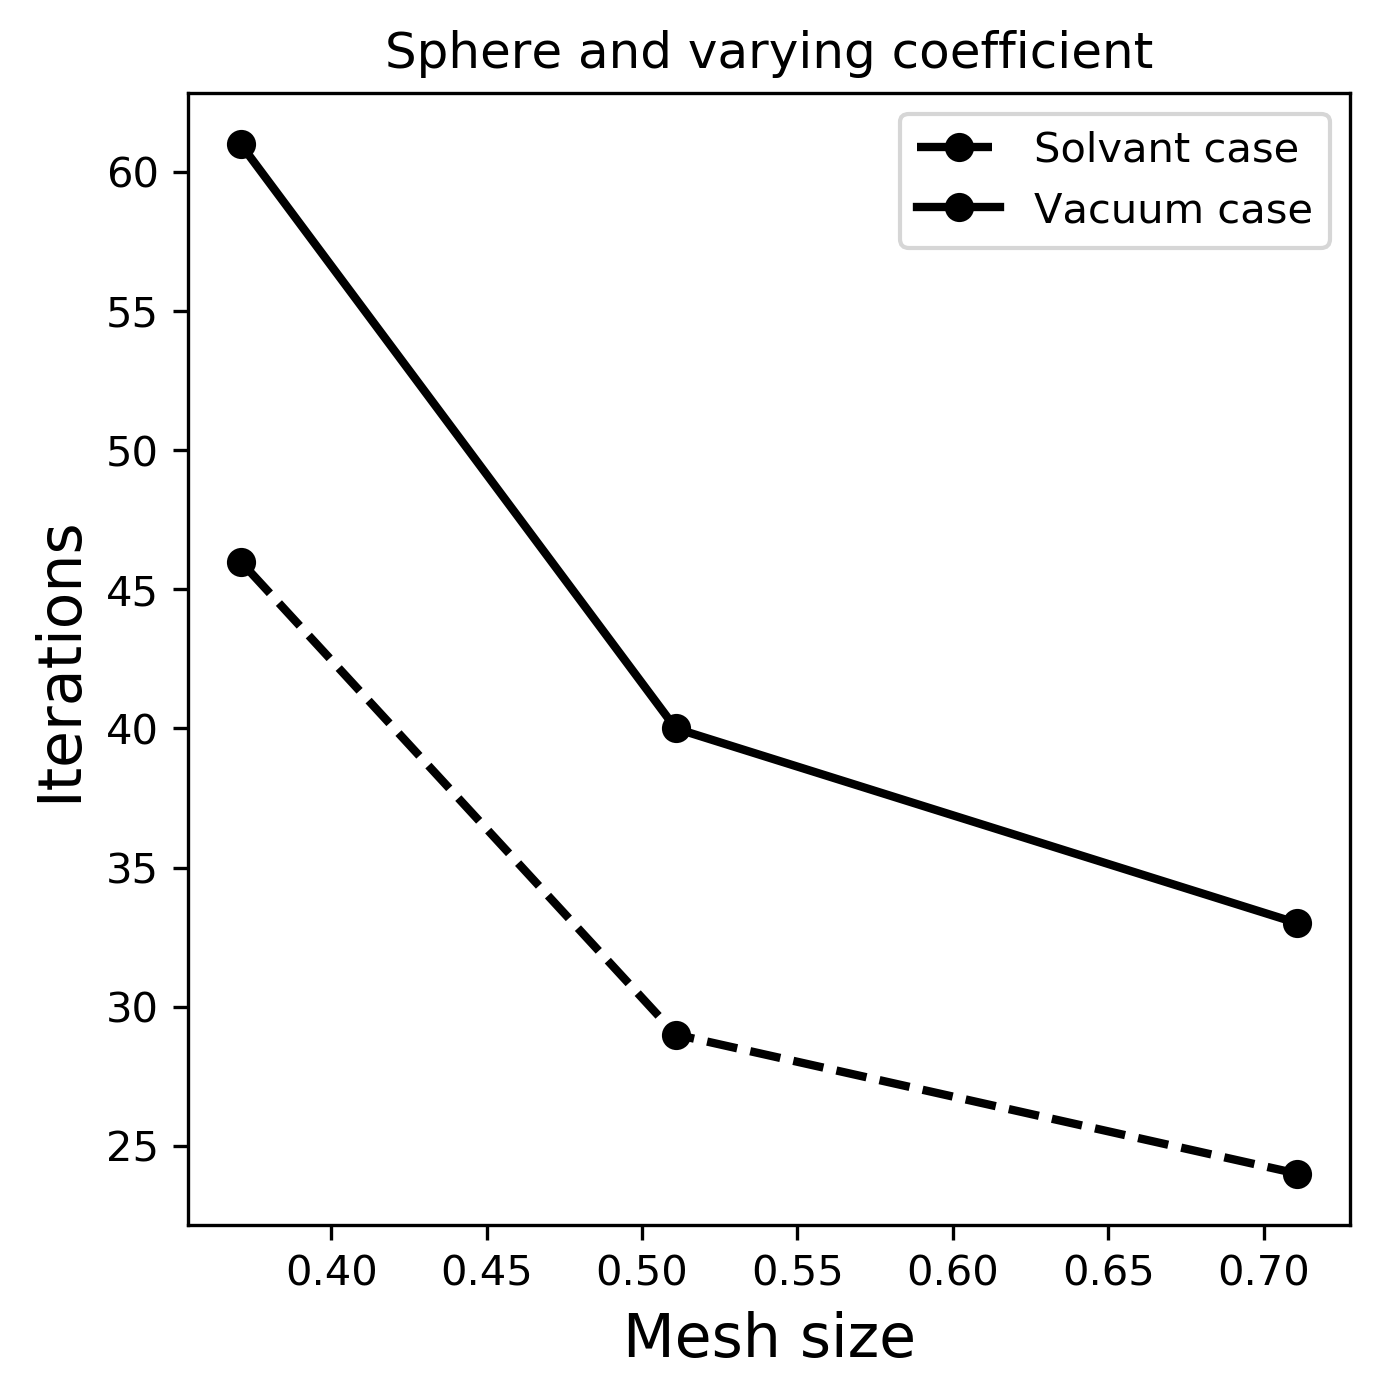
\includegraphics[width=\linewidth]{Hybrid_FEM_BEM_Sphere_varying_coeff_iter.png}
  \caption{Iterations}
\endminipage\hfill
\minipage{0.45\textwidth}%
  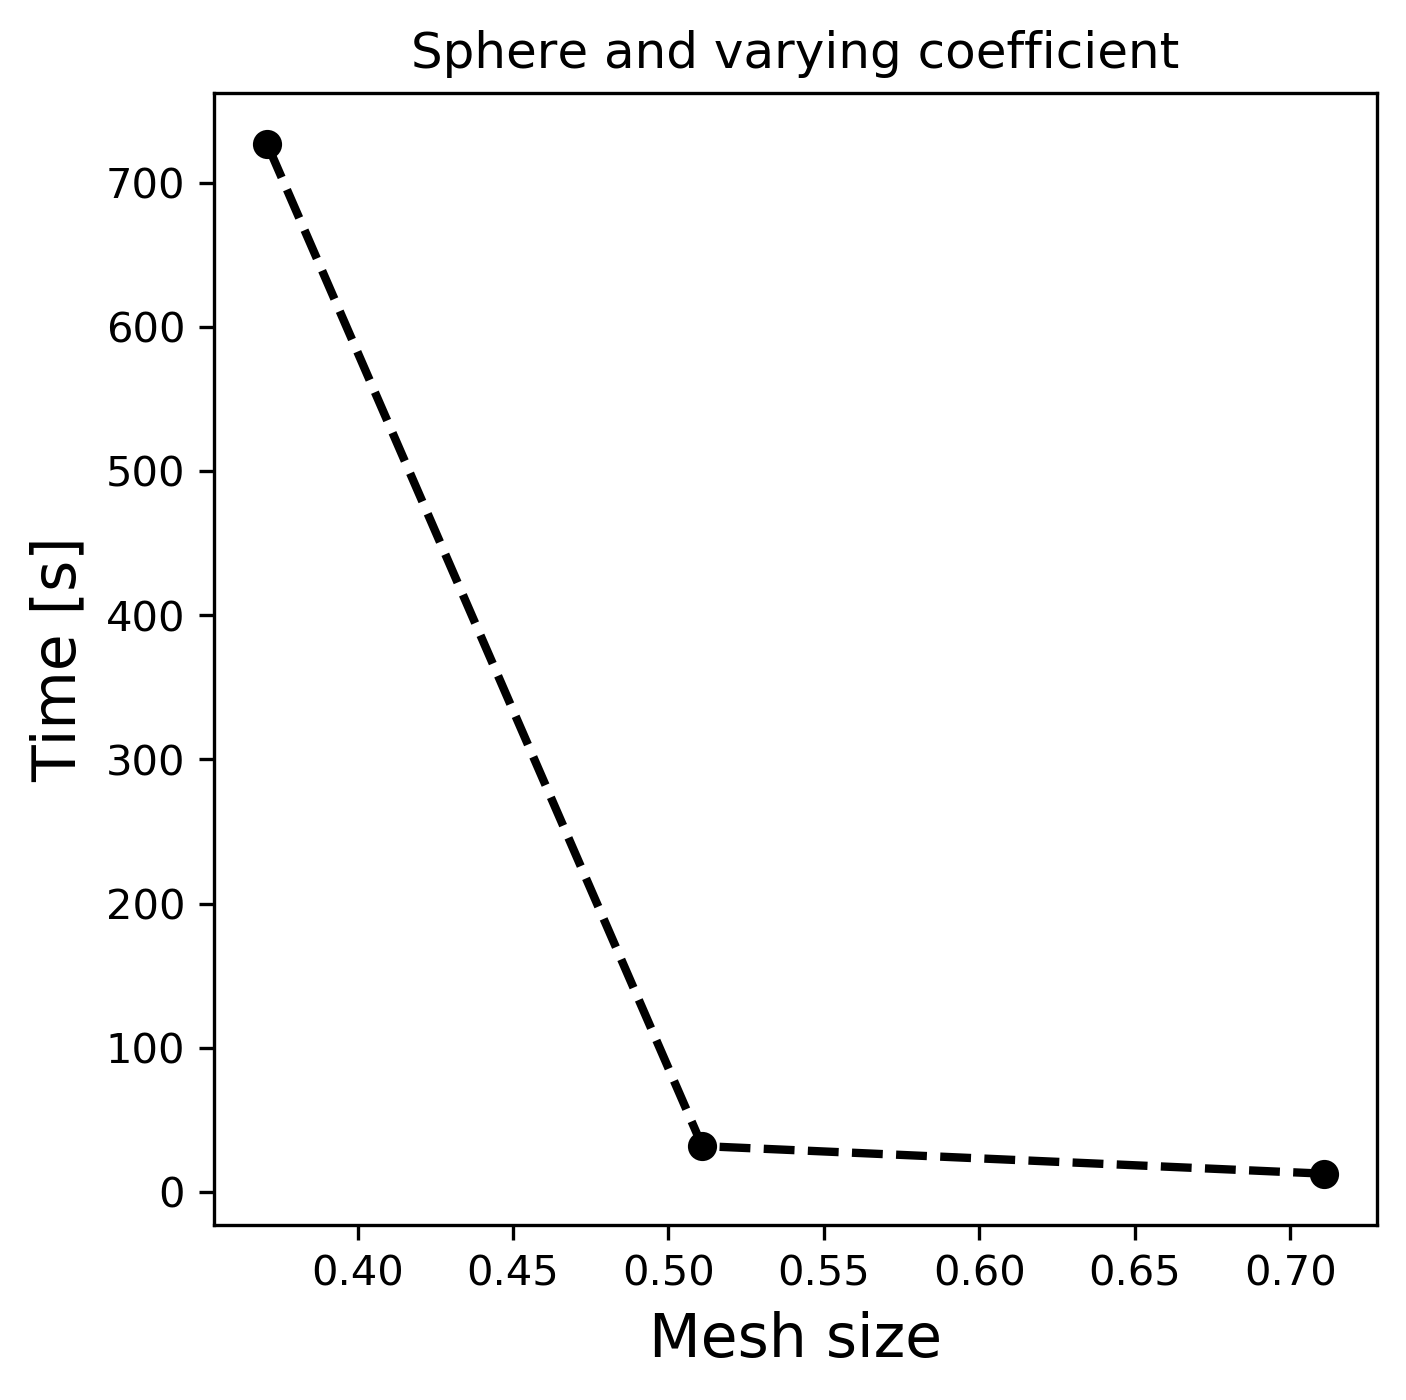
\includegraphics[width=\linewidth]{Hybrid_FEM_BEM_Sphere_varying_coeff_time.png}
  \caption{Computational time}
\endminipage
\end{figure}
    \end{itemize}

\subsection*{\sffamily \large Validation for a spherical cavity}

Compare solvation energy results of hybrid FEM-BEM with Delphi

\subsection*{\sffamily \large Convergence and performance for a molecular geometry}
\begin{itemize}
    \item Mesh refinement study using hybrid FEM-BEM and Delphi (if possible) on arginine or small protein. Check if they are converging to same result.
    \item Compare timings for equivalent error (if possible)
\end{itemize}

    \begin{itemize}
        \item Standard FEM-BEM
\begin{figure}[!htb]
\minipage{0.45\textwidth}
  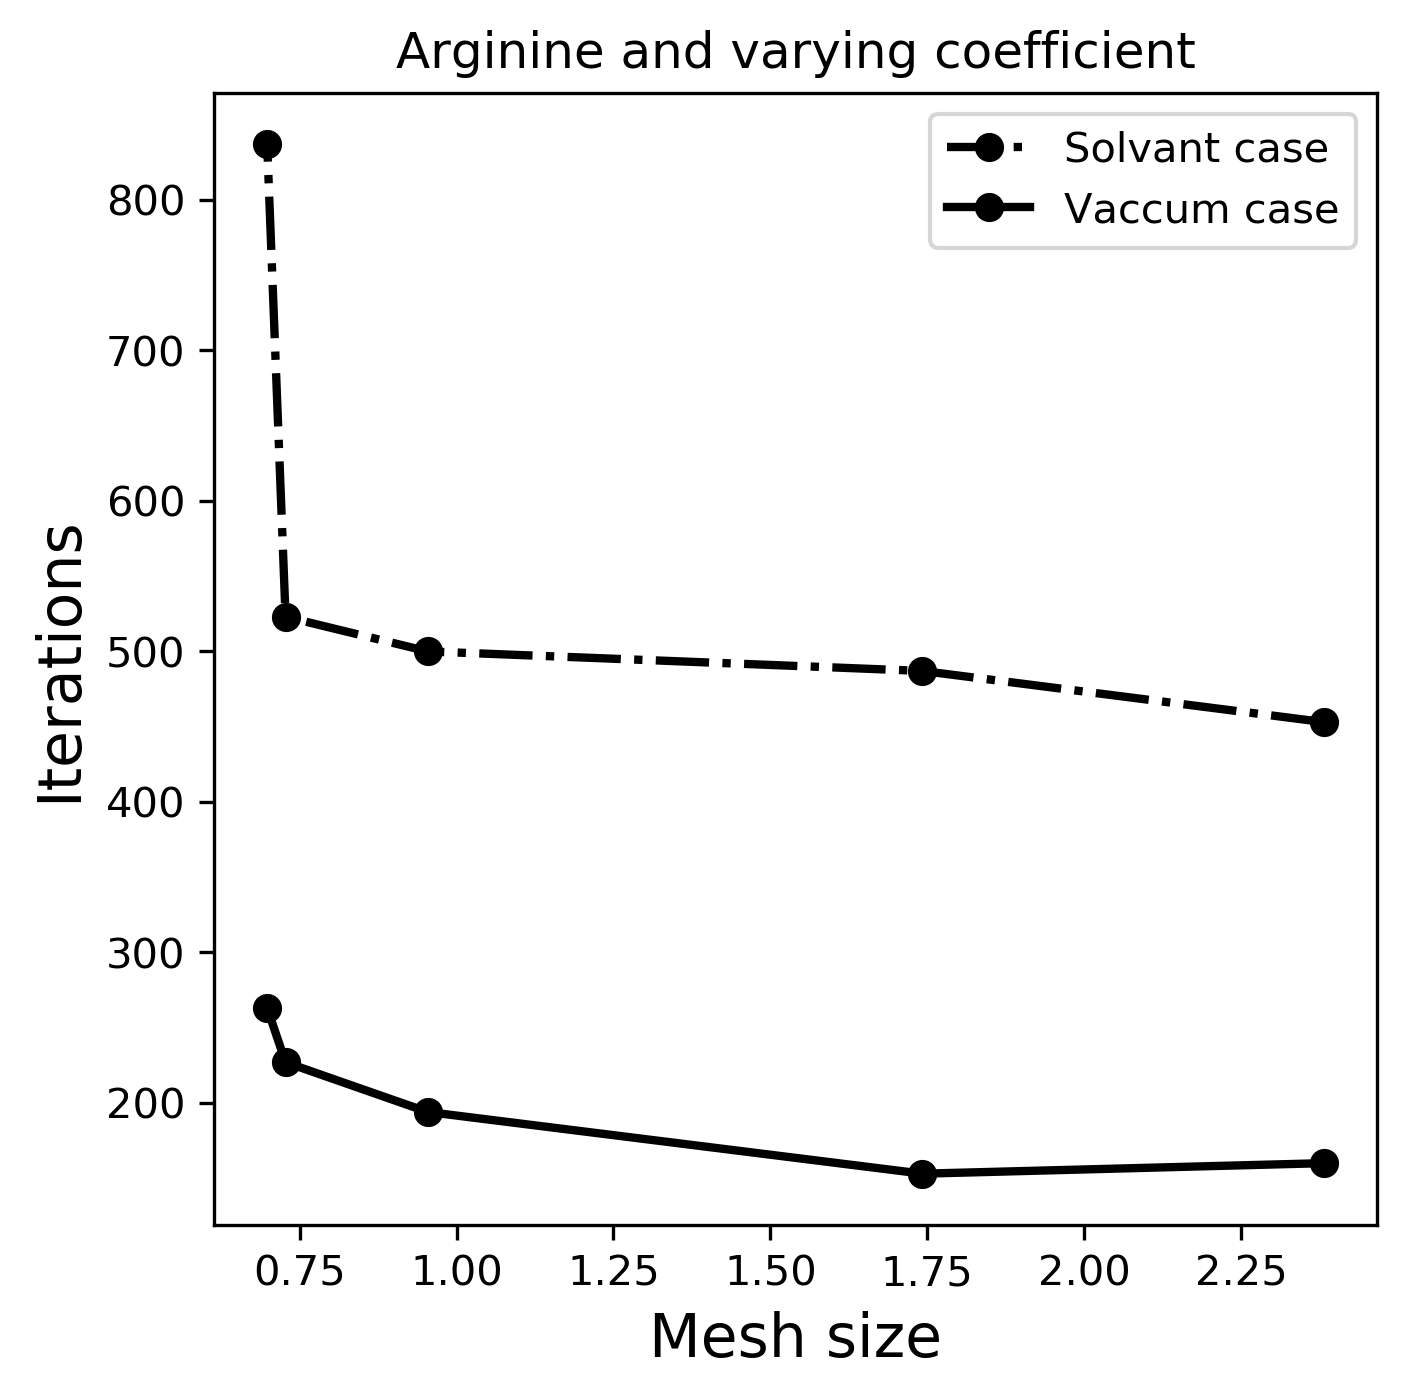
\includegraphics[width=\linewidth]{FEM_BEM_Arginine_varying_coeff_iter.png}
  \caption{Iterations}
\endminipage\hfill
\minipage{0.45\textwidth}%
  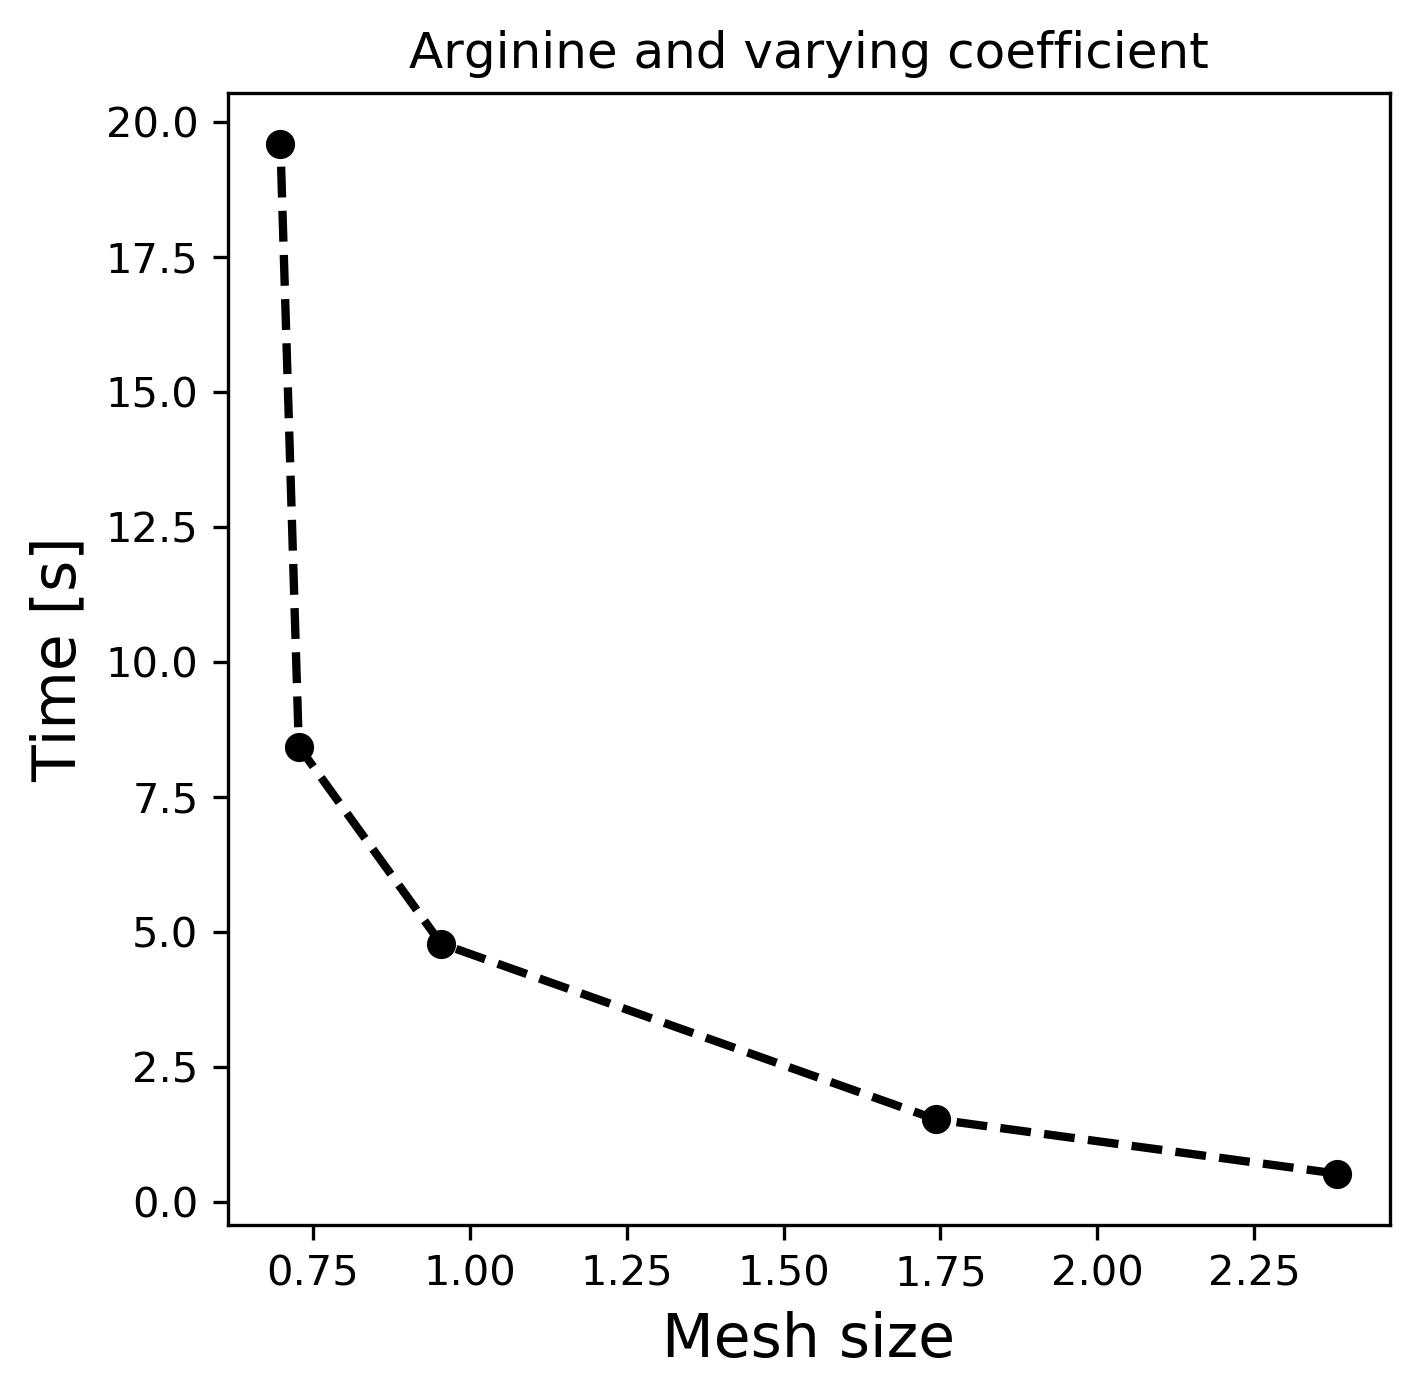
\includegraphics[width=\linewidth]{FEM_BEM_Arginine_varying_coeff_time.png}
  \caption{Computational time}
\endminipage
\end{figure}
        \item Hybrid FEM-BEM
\begin{figure}[!htb]
\minipage{0.45\textwidth}
  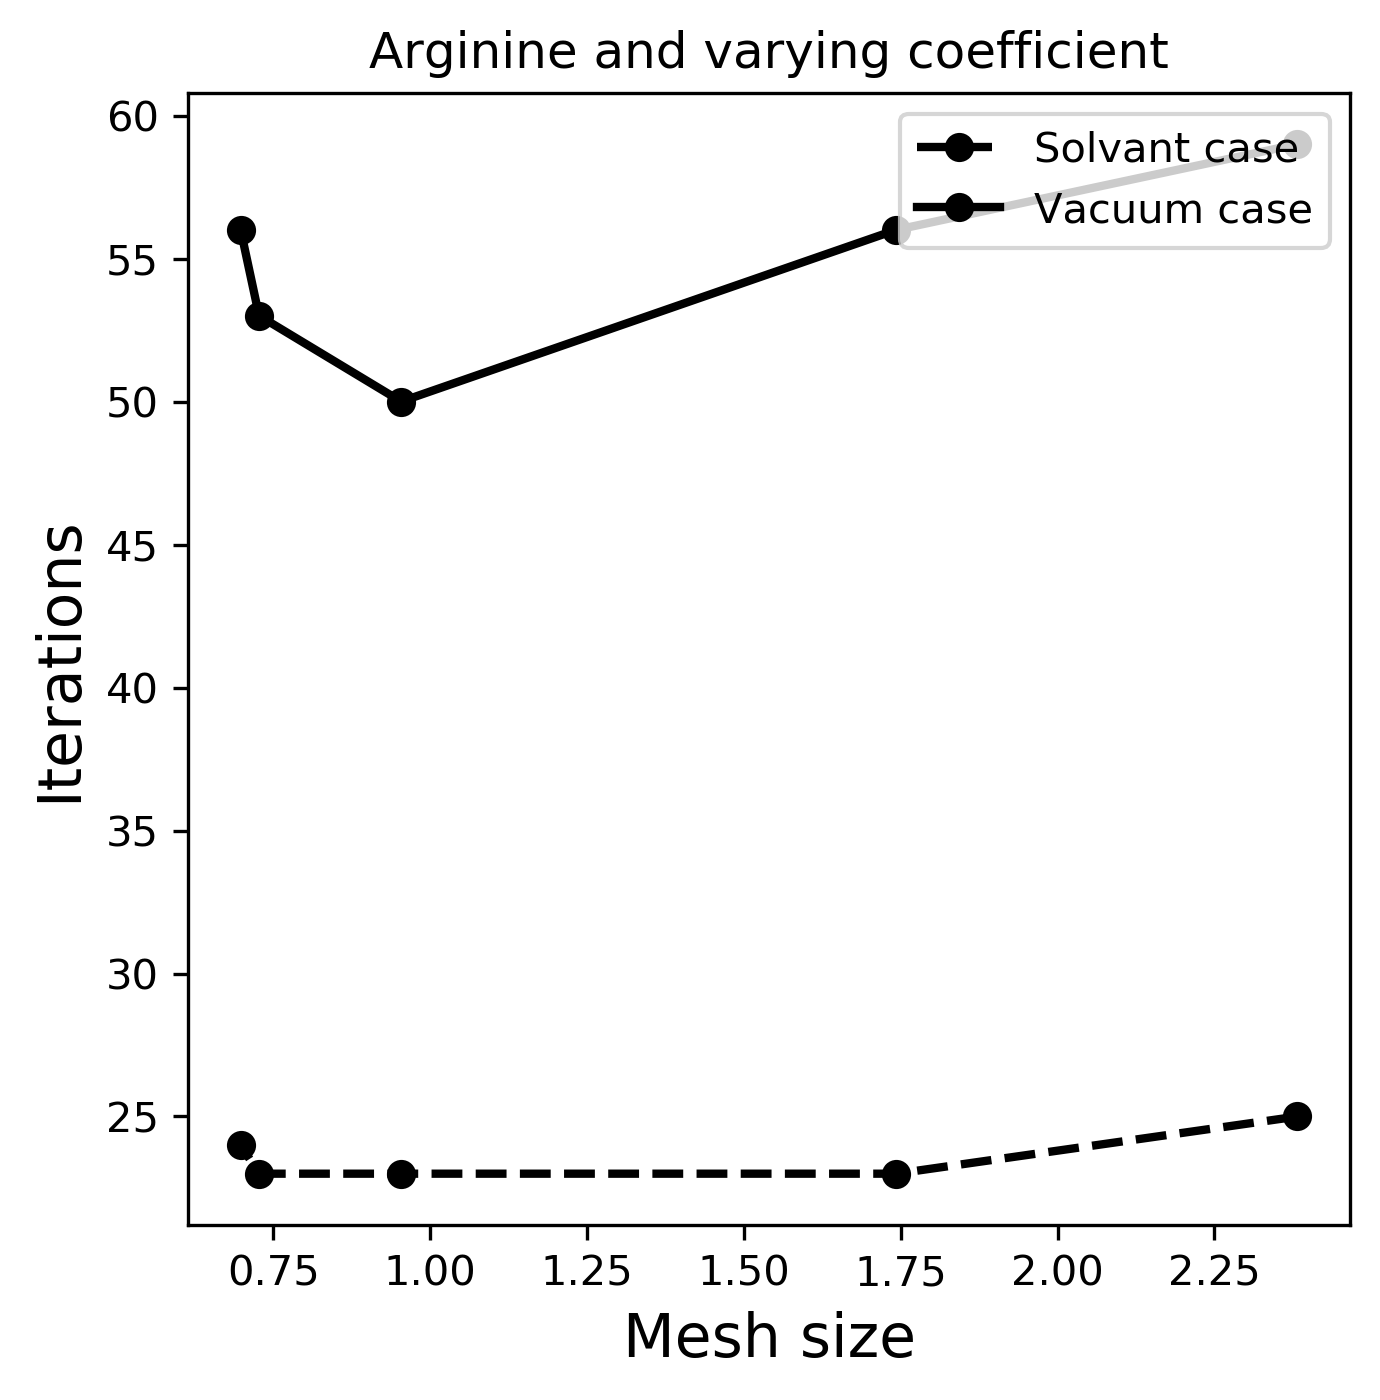
\includegraphics[width=\linewidth]{Hybrid_FEM_BEM_Arginine_varying_coeff_iter.png}
  \caption{Iterations}
\endminipage\hfill
\minipage{0.45\textwidth}%
  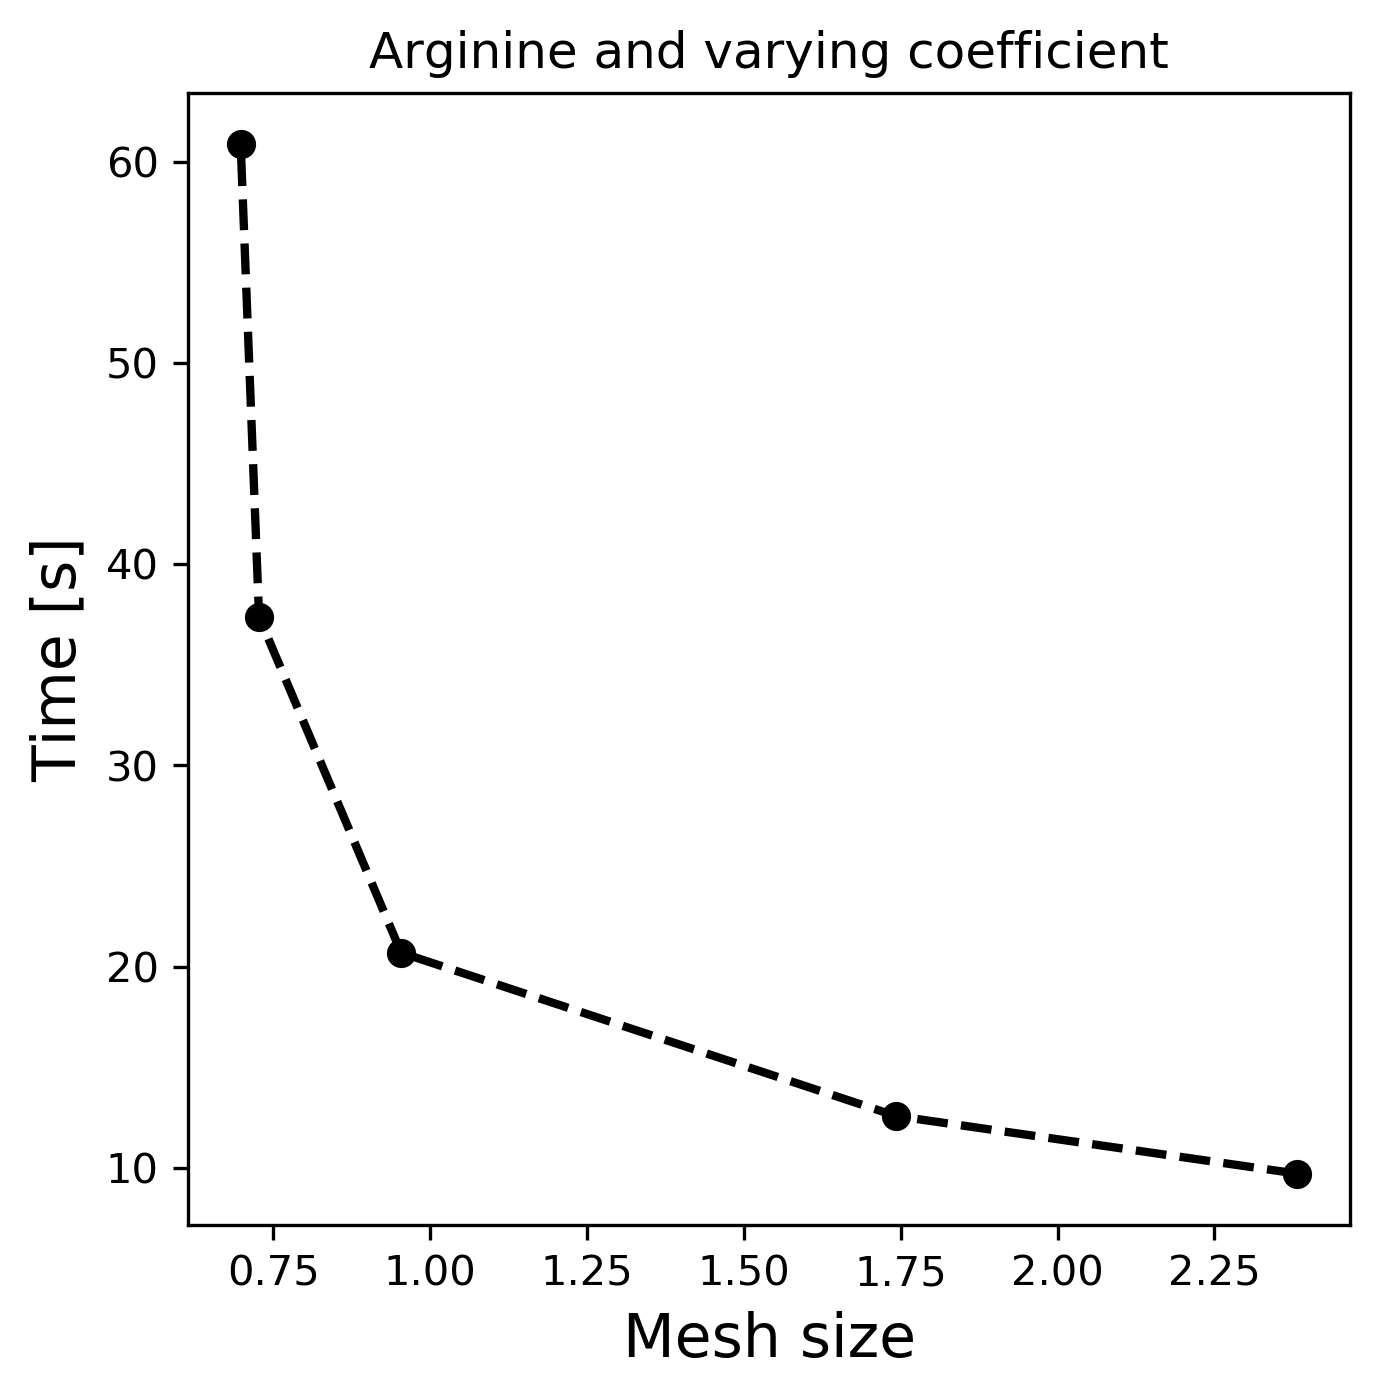
\includegraphics[width=\linewidth]{Hybrid_FEM_BEM_Arginine_varying_coeff_time.png}
  \caption{Computational time}
\endminipage
\end{figure}
    \end{itemize}

\subsection*{\sffamily \large Performance analysis for larger structures}

For a given mesh refinement, show solvation energy and timings using preconditioned hybrid FEM-BEM up to the biggest problem we can do on whatever computer we're using.
